% !TeX program = xelatex
% !TeX TXS-program:compile = txs:///xelatex/[--shell-escape]
%%%%%%%%%%%%%%%%%%%%%%%%%%%%%%%%%%%%%%%%%%%%%%%%%%%%%%%%%%%%%%%%%%%%%%%%
% Plantilla TFG/TFM
% Escuela Politécnica Superior de la Universidad de Alicante
% Realizado por: Jose Manuel Requena Plens
% Contacto: info@jmrplens.com / Telegram:@jmrplens
%%%%%%%%%%%%%%%%%%%%%%%%%%%%%%%%%%%%%%%%%%%%%%%%%%%%%%%%%%%%%%%%%%%%%%%%

% Elige si deseas optimizar la ejecución del proyecto almacenando las figuras generadas con TikZ y PGF en una carpeta (archivos/figuras-procesadas).
% 1 - Si, 2 - No
\def\OptimizaTikZ{1}

% Archivo .TEX que incluye todas las configuraciones del documento y los paquetes. Añade todo aquello que necesites utilizar en el documento en este archivo.
% En él se encuentra la configuración de los márgenes, establecidos según las directrices de estilo de la EPS.
%%%%%%%%%%%%%%%%%%%%%%%%%%%%%%%%%%%%%%%%%%%%%%%%%%%%%%%%%%%%%%%%%%%%%%%%
% Plantilla TFG/TFM
% Escuela Politécnica Superior de la Universidad de Alicante
% Realizado por: Jose Manuel Requena Plens
% Contacto: info@jmrplens.com / Telegram:@jmrplens
%%%%%%%%%%%%%%%%%%%%%%%%%%%%%%%%%%%%%%%%%%%%%%%%%%%%%%%%%%%%%%%%%%%%%%%%

%%%%%%%%%%%%%%%%%%%%%%%%
% FORMATO DEL DOCUMENTO
%%%%%%%%%%%%%%%%%%%%%%%%
% scrbook es la clase de documento
% Si se desea que no haya página en blanco entre capítulos añadir "openany" en los parámetros de la clase. Sino siempre los capítulos empezarán en página impar.
\documentclass[a4paper,11pt,titlepage]{scrbook}
\KOMAoption{toc}{bib,chapterentryfill} % Opciones del índice
\usepackage{scrhack} % Previene algunos errores
% Paquete de formato para scrbook. Con marcas, linea-separador superior e inferior
\usepackage[automark,headsepline,footsepline]{scrlayer-scrpage}
\usepackage{pifont}
\usepackage[utf8]{inputenc}
\usepackage{tcolorbox}
\clearpairofpagestyles		% Borra los estilos por defecto
%%
% Formato y contenido de la información de cabecera y pie de página
%%
% Información de capítulo en cabecera e interno
\ihead{{\color{gray30}\scshape\small\headmark}}	
% Número de página en cabecera y externo
\ohead{\normalfont\pagemark} 
% Número de página en pie de página y externo. Sólo en páginas sin cabecera
\ofoot[\normalfont\pagemark]{}
%% 		
% Edición del contenido de las distintas partes de la cabecera
%%
\renewcommand{\chaptermark}[1]{\markboth{#1}{}} % Capítulo (Solo texto)
\renewcommand{\sectionmark}[1]{\markright{\thesection. #1}} % Sección (Número y texto)
\setkomafont{pagenumber}{} % Número de página (Sin nada añadido)

% Añade al índice y numera hasta la profundidad 4.
% 1:section,2:subsection,3:subsubsection,4:paragraph
\setcounter{tocdepth}{4}
\setcounter{secnumdepth}{4}
% Muestra una regla para comprobar el formato de las páginas
%\usepackage[type=upperleft,showframe,marklength=8mm]{fgruler}
% MÁRGENES DE LAS PÁGINAS
\usepackage[
  inner	=	3.0cm, % Margen interior
  outer	=	2.5cm, % Margen exterior
  top	=	2.5cm, % Margen superior
  bottom=	2.5cm, % Margen inferior
  includeheadfoot, % Incluye cabecera y pie de página en los márgenes
]{geometry}
% Valor de interlineado
\renewcommand{\baselinestretch}{1.5} % 1.5 línea de interlineado
% Para poder generar páginas horizontales
\usepackage{lscape}
% Ancho de la zona para comentarios en el margen. (modificado para todonotes)
\setlength{\marginparwidth}{1.9cm}

%%%%%%%%%%%%%%%%%%%%%%%%
% BIBLIOGRAFÍA
%%%%%%%%%%%%%%%%%%%%%%%%
\usepackage{apacite} % NORMA APA
\usepackage{natbib}
\usepackage{breakcites}

%%%%%%%%%%%%%%%%%%%%%%%%
% DOCUMENTO EN ESPAÑOL
%%%%%%%%%%%%%%%%%%%%%%%%
\usepackage[base]{babel}
\usepackage{polyglossia}
\setdefaultlanguage{spanish}

\addto\captionsspanish{%
	\renewcommand{\listtablename}{Índice de tablas} 
	\renewcommand{\tablename}{Tabla}
	\renewcommand{\lstlistingname}{Código}
	\renewcommand{\lstlistlistingname}{Índice de \lstlistingname s}
	\renewcommand{\glossaryname}{Glosario}
	\renewcommand{\acronymname}{Acrónimos}
	\renewcommand{\bibname}{Bibliografía}%
}

%%%%%%%%%%%%%%%%%%%%%%%% 
% COLORES
%%%%%%%%%%%%%%%%%%%%%%%% 
% Biblioteca de colores
\usepackage{color}
\usepackage[dvipsnames]{xcolor}
% Otros colores definidos por el usuario
\definecolor{gray97}{gray}{.97}
\definecolor{gray75}{gray}{.75}
\definecolor{gray45}{gray}{.45}
\definecolor{gray30}{gray}{.30}
\definecolor{negro}{RGB}{0,0,0}
\definecolor{blanco}{RGB}{255,255,255}
\definecolor{dkgreen}{rgb}{0,.6,0}
\definecolor{dkblue}{rgb}{0,0,.6}
\definecolor{dkyellow}{cmyk}{0,0,.8,.3}
\definecolor{gray}{rgb}{0.5,0.5,0.5}
\definecolor{mauve}{rgb}{0.58,0,0.82}
\definecolor{deepblue}{rgb}{0,0,0.5}
\definecolor{deepred}{rgb}{0.6,0,0}
\definecolor{deepgreen}{rgb}{0,0.5,0}
\definecolor{MyDarkGreen}{rgb}{0.0,0.4,0.0}
\definecolor{bluekeywords}{rgb}{0.13,0.13,1}
\definecolor{greencomments}{rgb}{0,0.5,0}
\definecolor{redstrings}{rgb}{0.9,0,0}

%%%%%%%%%%%%%%%%%%%%%%%%
% TABLAS
%%%%%%%%%%%%%%%%%%%%%%%%
% Paquetes para tablas
\usepackage{longtable,booktabs,array,multirow,multicol,tabularx,ragged2e,array}
% Nuevos tipos de columna para tabla, se pueden utilizar como por ejemplo C{3cm} en la definición de columnas de la función tabular
\newcolumntype{L}[1]{>{\raggedright\let\newline\\\arraybackslash\hspace{0pt}}m{#1}}
\newcolumntype{C}[1]{>{\centering\let\newline\\\arraybackslash\hspace{0pt}}m{#1}}
\newcolumntype{R}[1]{>{\raggedleft\let\newline\\\arraybackslash\hspace{0pt}}m{#1}}

%%%%%%%%%%%%%%%%%%%%%%%% 
% GRAFICAS y DIAGRAMAS 
%%%%%%%%%%%%%%%%%%%%%%%% 
% Paquete para todo tipo de gráficas, diagramas, modificación de imágenes, etc
\usepackage{tikz,tikzpagenodes}
\usetikzlibrary{tikzmark,calc,shapes.geometric,arrows,backgrounds,shadings,shapes.arrows,shapes.symbols,shadows,positioning,fit,automata,patterns,intersections}
\usepackage{pgfplots}
\pgfplotsset{colormap/jet}
\pgfplotsset{compat=newest} % Compatibilidad
\usepgfplotslibrary{patchplots,groupplots,fillbetween,polar}
\usepackage{pgfplotstable}
% Guardar las figuras realizadas con Tikz y Pgf en una carpeta externa
% para agilizar el procesado y tenerlas para utilizarlas en otros
% documentos
\newif\ifOptimizaTikZ
\OptimizaTikZtrue % o \OptimizaTikZfalse para desactivarlo

\ifOptimizaTikZ
  \usepgfplotslibrary{external}
  \tikzexternalize[prefix=archivos/figuras-procesadas/] % Ruta
  \tikzset{%
    external/system call ={xelatex -enable-write18 -halt-on-error -interaction=batchmode -jobname "\image" "\texsource"},
  }
\fi


% Estilos para elementos graficos
% Cajas y cajas de texto
\tikzstyle{Caja1} = [green,very thick,rounded corners,fill=white, fill opacity=0.5]
\tikzstyle{Texto1} = [fill=white,thick,shape=circle,draw=black,inner sep=2pt,font=\sffamily,text=black]
\tikzstyle{Texto2} = [fill=white,thick,shape=rectangle,draw=black,inner sep=2pt,font=\sffamily,text=black]
\tikzstyle{Texto3} = [fill=white,thick,shape=circle,draw=black,inner sep=2pt,font=\sffamily,text=black]
% Cuadros de diagrama
\tikzstyle{rectvioleta} = [rectangle, rounded corners, text centered, draw=black, fill=blue!10]
\tikzstyle{rectnaranja} = [rectangle, minimum width=2cm, minimum height=1cm, text centered, draw=black, fill=orange!10]
\tikzstyle{romborosa} = [diamond, aspect=3, minimum width=3cm, minimum height=1cm, text centered, draw=black, fill=red!10]
\tikzstyle{rectverde} = [rectangle, minimum width=2cm, minimum height=1cm, text centered, draw=black, fill=green!10]
\tikzstyle{rectamarillo} = [rectangle, rounded corners, minimum width=2cm, minimum height=1cm, text centered, draw=black, fill=yellow!10]
% Flechas
\tikzstyle{arrow} = [thick,->,>=stealth]

%%%%%%%%%%%%%%%%%%%%%%%% 
% FIGURAS, TABLAS, ETC 
%%%%%%%%%%%%%%%%%%%%%%%% 
\usepackage{subcaption} % Para poder realizar subfiguras
\usepackage{caption} % Para aumentar las opciones de diseño
% Nombres de figuras, tablas, etc, en negrita la numeración, todo con letra small
\captionsetup{labelfont={bf,small},textfont=small}
% Paquete para modificar los espacios arriba y abajo de una figura o tabla
\usepackage{setspace}
% Define el espacio tanto arriba como abajo de las figuras, tablas
\setlength{\intextsep}{5mm}
% Para ajustar tamaños de texto de toda una tabla o grafica
% Uso: {\scalefont{0.8} \begin{...} \end{...} }
\usepackage{scalefnt}
% Redefine las tablas y figuras para eliminar el '.' entre la numeración y el texto
\renewcommand*{\figureformat}{\figurename~\thefigure}
\renewcommand*{\tableformat}{\tablename~\thetable}

%%%%%%%%%%%%%%%%%%%%%%%% 
% TEXTO
%%%%%%%%%%%%%%%%%%%%%%%%
% Paquete para poder modificar las fuente de texto
\usepackage{xltxtra}
% Cualquier tamaño de texto. Uso: {\fontsize{100pt}{120pt}\selectfont tutexto}
\usepackage{anyfontsize}
% Para modificar parametros del texto.
\usepackage{setspace}
% Paquete para posicionar bloques de texto
\usepackage{textpos}
% Paquete para realizar cajas de texto. 
% Uso: \begin{mdframed}[linecolor=red!100!black] tutexto \end{mdframed}
\usepackage{framed,mdframed}
% Para subrayar. Uso: \hlc[tucolor]{tutexto}
\newcommand{\hlc}[2][yellow]{ {\sethlcolor{#1} \hl{#2}} }

%%%%%%%%%%%%%%%%%%%%%%%% 
% OTROS
%%%%%%%%%%%%%%%%%%%%%%%%
% Para hacer una pagina horizontal. Uso: \begin{landscape} xxxx \end{lanscape}
\usepackage{lscape} 
% Para incluir paginas PDF. Uso:
% \includepdf[pages={1}]{tuarchivo.pdf}
\usepackage{pdfpages}
% Para introducir url's con formato. Uso: \url{http://www.google.es}
\usepackage{url}
% Amplia muchas funciones graficas de latex
\usepackage{graphicx}
% Paquete que añade el hipervinculo en referencias dentro del documento, indice, etc
% Se define sin bordes alrededor. Uso: \ref{tulabel}
\usepackage[pdfborder={000}]{hyperref}
\usepackage{float}
\usepackage{placeins}
\usepackage{afterpage}
\usepackage{verbatim}
% Paquete para condicionales avanzados
\usepackage{xstring,xifthen}
% Paquete para realizar calculos en el código
\usepackage{calc}
% Para rotar tablas o figuras o su contenido
\usepackage{rotating} 
% Para incluir comentarios en el texto. El parámetro 'disable' oculta todas las notas.
% USO: \todo{tutexto}
\usepackage[textsize=tiny,spanish,shadow,textwidth=2cm]{todonotes}
%\reversemarginpar % Descomentar si se quiere todos los comentarios en el mismo lado
\usepackage{listings}

\lstset{
    breaklines=true,
    breakatwhitespace=true,
    basicstyle=\ttfamily,
    keywordstyle=\color{blue},
    frame=single,
    postbreak=\mbox{\textcolor{red}{$\hookrightarrow$}\space}
}

% Desactiva la exportación de los ToDo y Missingfigures como figuras
\if\OptimizaTikZ 1
\makeatletter
\renewcommand{\todo}[2][]{\tikzexternaldisable\@todo[#1]{#2}\tikzexternalenable}
\makeatother
\usepackage{letltxmacro}
\LetLtxMacro{\oldmissingfigure}{\missingfigure}
\makeatletter
\renewcommand{\missingfigure}[2][]{\tikzexternaldisable\oldmissingfigure[{#1}]{#2}\tikzexternalenable}
\makeatother
\fi

%%%%%%%%%%%%%%%%%%%%%%%% 
% GLOSARIOS
%%%%%%%%%%%%%%%%%%%%%%%%
\usepackage[acronym,nonumberlist,toc]{glossaries}
\usepackage{glossary-superragged}
\newglossarystyle{modsuper}{%
  \setglossarystyle{super}%
  \renewcommand{\glsgroupskip}{}
}
\renewcommand{\glsnamefont}[1]{\textbf{#1}}


%%%%%%%%%%%%%%%%%%%%%%%% 
% COMANDOS AÑADIDOS
%%%%%%%%%%%%%%%%%%%%%%%%
% Para mostrar la fecha actual (mes año) con \Hoy
\newcommand{\MES}{%
  \ifcase\month% 0
    \or Enero% 1
    \or Febrero% 2
    \or Marzo% 3
    \or Abril% 4
    \or Mayo% 5
    \or Junio% 6
    \or Julio% 7
    \or Agosto% 8
    \or Septiembre% 9
    \or Octubre% 10
    \or Noviembre% 11
    \or Diciembre% 12
  \fi}
\newcommand{\ANYO}{\number\year}
\newcommand{\Hoy}{\MES\ \ANYO}

%%%%%%%%%%%%%%%%%%%%%%%% 
% MATEMÁTICAS
%%%%%%%%%%%%%%%%%%%%%%%%
\usepackage{mathtools,amsthm,amsfonts,amssymb,bm,mathrsfs,nicefrac,upgreek,bigints} 
% Comando para añadir información de variables a las ecuaciones
% Uso: \begin{condiciones}[donde:] ....... \end{condiciones}
\newenvironment{condiciones}[1][2]
  {%
   #1\tabularx{\textwidth-\widthof{#1}}[t]{
     >{$}l<{$} @{}>{${}}c<{{}$}@{} >{\raggedright\arraybackslash}X
   }%
  }
  {\endtabularx\\[\belowdisplayskip]}

%%%%%
% PARÁMETROS DE FORMATO DE CODIGOS
%%%%%
% Puedes editar los formatos para ajustarlos a tu gusto
%%%%%%%%%%%%%%%%%%%%%%%%%%%%%%%%%%%%%%%%%%%%%%%%%%%%%%%%%%%%%%%%%%%%%%%%
% Plantilla TFG/TFM
% Escuela Politécnica Superior de la Universidad de Alicante
% Realizado por: Jose Manuel Requena Plens
% Contacto: info@jmrplens.com / Telegram:@jmrplens
%%%%%%%%%%%%%%%%%%%%%%%%%%%%%%%%%%%%%%%%%%%%%%%%%%%%%%%%%%%%%%%%%%%%%%%%


%%%%%%%%%%%%%%%%%%%%%%%% 
% CÓDIGO. CONFIGURACIÓN. En el siguiente bloque están los estilos.
%%%%%%%%%%%%%%%%%%%%%%%%
% Paquete para mostrar código de matlab. En caja y lineas numeradas
\usepackage[framed,numbered]{matlab-prettifier}
% Paquete mostrar código de programación de distintos lenguajes
\usepackage{listings}
\lstset{ inputencoding=utf8,
extendedchars=true,
frame=single, % Caja donde se ubica el código
backgroundcolor=\color{gray97}, % Color del fondo de la caja
rulesepcolor=\color{black},
boxpos=c,
abovecaptionskip=-4pt,
aboveskip=12pt,
belowskip=0pt,
lineskip=0pt,
framerule=0pt,
framextopmargin=4pt,
framexbottommargin=4pt,
framexleftmargin=11pt,
framexrightmargin=0pt,
linewidth=\linewidth,
xleftmargin=\parindent,
framesep=0pt,
rulesep=.4pt,
stringstyle=\ttfamily,
showstringspaces = false,
showspaces = false,
showtabs = false,
columns=fullflexible,
basicstyle=\small\ttfamily,
commentstyle=\color{gray45},
keywordstyle=\bfseries,
tabsize=4,
numbers=left,
numbersep=1pt,
numberstyle=\tiny\ttfamily\color{gray75},
numberfirstline = false,
breaklines=true,
postbreak=\mbox{\textcolor{red}{$\hookrightarrow$}\space}, % Flecha al saltar de linea
prebreak=\mbox{\textcolor{red}{$\hookleftarrow$}\space}, % Flecha al saltar de linea
literate=
  {á}{{\'a}}1 {é}{{\'e}}1 {í}{{\'i}}1 {ó}{{\'o}}1 {ú}{{\'u}}1
  {Á}{{\'A}}1 {É}{{\'E}}1 {Í}{{\'I}}1 {Ó}{{\'O}}1 {Ú}{{\'U}}1
  {à}{{\`a}}1 {è}{{\`e}}1 {ì}{{\`i}}1 {ò}{{\`o}}1 {ù}{{\`u}}1
  {À}{{\`A}}1 {È}{{\'E}}1 {Ì}{{\`I}}1 {Ò}{{\`O}}1 {Ù}{{\`U}}1
  {ä}{{\"a}}1 {ë}{{\"e}}1 {ï}{{\"i}}1 {ö}{{\"o}}1 {ü}{{\"u}}1
  {Ä}{{\"A}}1 {Ë}{{\"E}}1 {Ï}{{\"I}}1 {Ö}{{\"O}}1 {Ü}{{\"U}}1
  {â}{{\^a}}1 {ê}{{\^e}}1 {î}{{\^i}}1 {ô}{{\^o}}1 {û}{{\^u}}1
  {Â}{{\^A}}1 {Ê}{{\^E}}1 {Î}{{\^I}}1 {Ô}{{\^O}}1 {Û}{{\^U}}1
  {œ}{{\oe}}1 {Œ}{{\OE}}1 {æ}{{\ae}}1 {Æ}{{\AE}}1 {ß}{{\ss}}1
  {ű}{{\H{u}}}1 {Ű}{{\H{U}}}1 {ő}{{\H{o}}}1 {Ő}{{\H{O}}}1
  {ç}{{\c c}}1 {Ç}{{\c C}}1 {ø}{{\o}}1 {å}{{\r a}}1 {Å}{{\r A}}1
  {€}{{\euro}}1 {£}{{\pounds}}1 {«}{{\guillemotleft}}1
  {»}{{\guillemotright}}1 {ñ}{{\~n}}1 {Ñ}{{\~N}}1 {¿}{{?`}}1,
  }

% Intenta no dividir los códigos en diferentes paginas si es posible
\lstnewenvironment{listing}[1][]
   {\lstset{#1}\pagebreak[0]}{\pagebreak[0]}

% Formato de títulos de los códigos
\DeclareCaptionFont{white}{\color{white}}
\DeclareCaptionFormat{listing}{\colorbox{gray}{\parbox{\textwidth - 2\fboxsep}{#1#2#3}}}
\captionsetup[lstlisting]{format=listing,labelfont=white,textfont=white,font= scriptsize}


%%%%%%%%%%%%%%%%%%%%%%%% 
% CÓDIGO. ESTILOS. Ajústalos a tu gusto
%%%%%%%%%%%%%%%%%%%%%%%%
\lstdefinestyle{Consola}
	{
	basicstyle=\scriptsize\bfseries\ttfamily,
	}
   
\lstdefinestyle{C}
	{
	basicstyle=\scriptsize,
	language=C,
	}
\lstdefinestyle{C-color}
	{
  	breaklines=true,
  	language=C,
  	basicstyle=\scriptsize,
  	keywordstyle=\bfseries\color{green!40!black},
  	commentstyle=\itshape\color{purple!40!black},
  	identifierstyle=\color{blue},
  	stringstyle=\color{orange},
    }
\lstdefinestyle{CSharp}
	{
	basicstyle=\scriptsize,
	language=[Sharp]C,
	escapeinside={(*@}{@*)},
	keywordstyle=\bfseries,
	}
\lstdefinestyle{CSharp-color}
	{
	basicstyle=\scriptsize,
	language=[Sharp]C,
	escapeinside={(*@}{@*)},
	commentstyle=\color{greencomments},
	keywordstyle=\color{bluekeywords}\bfseries,
	stringstyle=\color{redstrings},
	}
\lstdefinestyle{C++}
	{
	basicstyle=\scriptsize,
	language=C++,
 	}
 	
\lstdefinestyle{C++-color}
	{
  	breaklines=true,
  	language=C++,
  	basicstyle=\scriptsize,
  	keywordstyle=\bfseries\color{green!40!black},
  	commentstyle=\itshape\color{purple!40!black},
  	identifierstyle=\color{blue},
  	stringstyle=\color{orange},
    }
    
\lstdefinestyle{PHP}
	{
	basicstyle=\scriptsize,
	language=PHP,
	}
	
\lstdefinestyle{PHP-color}
	{
	basicstyle=\scriptsize,
	language=PHP,
	keywordstyle    = \color{dkblue},
  	stringstyle     = \color{red},
  	identifierstyle = \color{dkgreen},
  	commentstyle    = \color{gray},
  	emph            =[1]{php},
  	emphstyle       =[1]\color{black},
  	emph            =[2]{if,and,or,else},
  	emphstyle       =[2]\color{dkyellow}
  }
  
\lstdefinestyle{Matlab}
	{
	basicstyle=\scriptsize,
	language=Matlab,
	numberstyle=\tiny\ttfamily\color{gray75},
	}
	
\lstdefinestyle{Matlab-color}
	{
	style = Matlab-editor,
	basicstyle=\scriptsize,
	numberstyle=\tiny\ttfamily\color{gray75},
	}
	
\lstdefinestyle{Latex}
	{
	language=[LaTeX]{Tex},
    basicstyle=\scriptsize,
    literate={\$}{{{\bfseries\$}}}1,
    alsoletter={\\,*,\&},
    emph =[1]{\\begin,\\end,\\caption,\\label,\\centering,\\FloatBarrier,
              \\lstinputlisting,\\scalefont,\\addplot,\\input,
              \\legend,\\item,\\subitem,\\includegraphics,\\textwidth,
              \\section,\\subsection,\\subsubsection,\\paragraph,
              \\cite,\\citet,\\citep,\\gls,\\bibliographystyle,\\url,
              \\citet*,\\citep*,\\todo,\\missingfigure,\\footnote},
  	emphstyle =[1]\bfseries,
  	emph = [2]{equation,subequations,eqnarray,figure,subfigure,
  			   condiciones,flalign,tikzpicture,axis,lstlisting,
  			   itemize,description
  			   },
  	emphstyle =[2]\bfseries,
    numbers=none,
	}
	
\lstdefinestyle{Latex-color}
	{
	language=[LaTeX]{Tex},
    basicstyle=\scriptsize,
    commentstyle=\color{dkgreen},
    identifierstyle=\color{black},
    literate={\$}{{{\bfseries\color{Dandelion}\$}}}1, % Colorea el simbolo dollar
    alsoletter={\\,*,\&},
    emph =[1]{\\begin,\\end,\\caption,\\label,\\centering,\\FloatBarrier,
              \\lstinputlisting,\\scalefont,\\addplot,\\input,
              \\legend,\\item,\\subitem,\\includegraphics,\\textwidth,
              \\section,\\subsection,\\subsubsection,\\paragraph,
              \\cite,\\citet,\\citep,\\gls,\\bibliographystyle,\\url,
              \\citet*,\\citep*,\\todo,\\missingfigure,\\footnote},
  	emphstyle =[1]\bfseries\color{RoyalBlue},
  	emph = [2]{equation,subequations,eqnarray,figure,subfigure,
  			   condiciones,flalign,tikzpicture,axis,lstlisting,
  			   itemize,description
  			   },
  	emphstyle =[2]\bfseries,
    numbers=none,
	}
\lstdefinestyle{Java}
{
	basicstyle=\scriptsize,
	language=Java,
}

\lstdefinestyle{Java-color}
{
	basicstyle=\scriptsize,
	language=Java,
  	keywordstyle=\color{blue},
  	commentstyle=\color{dkgreen},
  	stringstyle=\color{mauve},
}
\lstdefinestyle{Python}
{
	language=Python,
	basicstyle=\scriptsize,
	otherkeywords={self},  
	keywordstyle=\bfseries,     
	emphstyle=\bfseries,    
	emph={MyClass,__init__},         
}

\lstdefinestyle{Python-color}
{
	language=Python,
	basicstyle=\scriptsize,
	otherkeywords={self},          
	keywordstyle=\bfseries\color{deepblue},
	emph={MyClass,__init__},         
	emphstyle=\bfseries\color{deepred},    
	stringstyle=\color{deepgreen},
}
\lstdefinestyle{R}
{
	language=R,                     
  	basicstyle=\scriptsize,
  	keywordstyle=\bfseries, 
}
\lstdefinestyle{R-color}
{
	language=R,                     
  	basicstyle=\scriptsize,
  	keywordstyle=\bfseries\color{RoyalBlue}, 
  	commentstyle=\color{YellowGreen},
  	stringstyle=\color{ForestGreen}  
}


%%%%%
% DEFINICION DE CONCEPTOS
%%%%
% Uso ejemplo: \begin{ejemplo} tucontenido \end{ejemplo} 
\newtheorem{teorema}{Teorema}[chapter]
\newtheorem{ejemplo}{Ejemplo}[chapter]
\newtheorem{definicion}{Definición}[chapter]



%%%%%%%%%%%%%%%%%%%%%%%%%%%%%%%%%%%%%%%%%%%%%%%%%%%%%%%%%%%%%%%%%%%%%%
% INFORMACIÓN DEL TFG
% Comentar lo que NO se desee añadir y sustituir con la información correcta.
%%%%%%%%%%%%%%%%%%%%%%%%%%%%%%%%%%%%%%%%%%%%%%%%%%%%%%%%%%%%%%%%%%%%%%
% Título y subtítulo
\newcommand{\titulo}{Plataforma de análisis de resultados de aprendizaje para fútbol base}
\newcommand{\subtitulo}{Trabajo Fin de Grado}
% Datos del autor
\newcommand{\miNombre}{Jorge Moreno Ozores}
% Determinar género para etiquetas Autore/Autora/Autor (nb o en blanco,f,m)
\newcommand{\miGenero}{m}
\newcommand{\miEmail}{jmo51@alu.ua.es}
% Datos del tutor/es
% Si no hay tutorB, comentar tutorB y dptoB para que la etiqueta sea Tutor:
\newcommand{\miTutor}{Virgilio Gilart Iglesias}
\newcommand{\miTutorB}{Diego Marcos Jorquera}
\newcommand{\departamentoTutor}{Tecnología Informática Y Computación}
\newcommand{\departamentoTutorB}{Tecnología Informática Y Computación}
% Datos de la facultad y universidad
\newcommand{\miFacultad}{Escuela Politécnica Superior}
\newcommand{\miFacultadCorto}{EPS UA}
\newcommand{\miUniversidad}{\protect{Universidad de Alicante}}
\newcommand{\miUbicacion}{Alicante}

%%%%%%%%%%%%%%%%%%%%%%%%%%%%%%%%%%%%%%%%%%%%%%%%%%%%%%%%%%%%%%%%%%%%%%
% INDICA TU TITULACIÓN
% ID	GRADO -------------------------------------------------
% 1		Ingeniería en Imagen y Sonido en Telecomunicación
% 2		Ingeniería Civil
% 3		Ingeniería Química
% 4		Ingeniería Informática
% 5		Ingeniería Multimedia
% 6		Arquitectura Técnica
% 7		Arquitectura
% 8		Robótica
% %		%%%%%%%%%%%%
% ID	MÁSTER ------------------------------------------------
% A		Telecomunicación
% B		Caminos, Canales y Puertos
% C		Gestión en la Edificación
% D		Desarrollo Web
% E		Materiales, Agua, Terreno
% F		Informática
% G 	Automática y Robótica
% H		Prevención de riesgos laborales
% I		Gestión Sostenible Agua
% J		Desarrollo Aplicaciones Móviles
% K		Ingeniería Química
% L		Ciberseguridad
% M		Ingeniería Geológica
%%%%%%%%%%%%%%%%%%%%%%%%%%%%%%%%%%%%%%%%%%%%%%%%%%%%%%%%%%%%%%%%%%%%%%%%%
%!!!!!!!!!!!!!!!!!!!!!!!!!!!!!!!!!!!!!!!!!!!!!!!!!!!!!!!!!!!!!!!!!!!!!%%%
																		%
\def\IDtitulo{4} % INTRODUCE LA ID DE TU TITULACIÓN						%
																		%
%!!!!!!!!!!!!!!!!!!!!!!!!!!!!!!!!!!!!!!!!!!!!!!!!!!!!!!!!!!!!!!!!!!!!!%%%
%%%%%%%%%%%%%%%%%%%%%%%%%%%%%%%%%%%%%%%%%%%%%%%%%%%%%%%%%%%%%%%%%%%%%%%%%

% Configuración automática según el identificador elegido
%%%%%%%%%%%%%%%%%%%%%%%%%%%%%%%%%%%%%%%%%%%%%%%%%%%%%%%%%%%%%%%%%%%%%%%%
% Plantilla TFG/TFM
% Escuela Politécnica Superior de la Universidad de Alicante
% Realizado por: Jose Manuel Requena Plens
% Contacto: info@jmrplens.com / Telegram:@jmrplens
%%%%%%%%%%%%%%%%%%%%%%%%%%%%%%%%%%%%%%%%%%%%%%%%%%%%%%%%%%%%%%%%%%%%%%%%

%%%%%%%%%%%%%%%%%%%%%%%% 
% COLORES DE GRADOS.
% Si el color de la titulación ha cambiado, modifícalo en las lineas siguientes.
%%%%%%%%%%%%%%%%%%%%%%%%
% Grados
\definecolor{teleco}{RGB}{32,2,116}			% Teleco
\definecolor{civil}{RGB}{201,56,140}			% Civil
\definecolor{quimica}{RGB}{41,199,255}		% Química
\definecolor{informatica}{RGB}{0,128,255}	% Informatica
\definecolor{multimedia}{RGB}{239,206,53}	% Multimedia
\definecolor{arquitecnica}{RGB}{0,179,148}	% Arquitectura técnica
\definecolor{arquitectura}{RGB}{181,0,0}		% Arquitectura
\definecolor{robotica}{RGB}{255,255,128}		% Robótica
% Másteres
\definecolor{masterteleco}{RGB}{32,2,116}	% Teleco
\definecolor{caminos}{RGB}{201,56,140}		% Caminos, Canales y Puertos
\definecolor{gestedif}{RGB}{50,120,50}		% Gestión Edificación
\definecolor{desweb}{RGB}{250,43,22}			% Desarrollo Web
\definecolor{mataguaterre}{RGB}{210,250,50}	% Materiales, Agua, Terreno
\definecolor{masterinfor}{RGB}{0,128,255}	% Informática
\definecolor{autorobo}{RGB}{83,145,201}		% Automática y Robótica
\definecolor{prevencion}{RGB}{0,100,0}		% Prevención Riesgos
\definecolor{gestionagua}{RGB}{7,138,197}	% Gestión Agua
\definecolor{moviles}{RGB}{121,11,21}		% Aplicaciones Móviles
\definecolor{masterquimica}{RGB}{41,199,255}	% Quimica
\definecolor{ciberseguridad}{RGB}{9,111,192}	% Ciberseguridad
\definecolor{geologica}{RGB}{245,125,0}		% Ingeniería Geológica

% Logotipos comunes de todas las titulaciones
\newcommand{\logoFacultad}{include/logos-universidad/LogoEPSNegro}
\newcommand{\logoUniversidad}{include/logos-universidad/LogoUANegro}
\newcommand{\logoUniversidadPortada}{include/logos-universidad/LogoUABlanco}

% Colores generales
\definecolor{negro}{RGB}{0,0,0}
\definecolor{blanco}{RGB}{255,255,255}
%%%%%%%%%%%%%%%%%%%%%%%% 
% CONDICIONALES. SEGUN LA ID ELEGIDA EN EL .TEX PRINCIPAL
% Según el ID seleccionado en TFG_EPS_UA.tex se configurará el nombre de la titulación, logotipos y color.
% Si tu titulación no esta correctamente definida cambia las imágenes que se definen para tu titulación en las lineas de abajo
% Si deseas añadir mas titulaciones ve al final de este archivo
%%%%%%%%%%%%%%%%%%%%%%%%
% Grados
	\if\IDtitulo 1 % Teleco
		% Logos
		\newcommand{\logoFacultadPortada}{include/logos-universidad/LogoEPSBlanco}
		\newcommand{\logoGradoPortada}{include/logos-titulaciones/LogoTelecoBlanco}
		\newcommand{\logoGrado}{include/logos-titulaciones/LogoTelecoNegro}
		% Texto
		\newcommand{\miGrado}{Grado en Ingeniería en Sonido e Imagen en Telecomunicación}
		\newcommand{\tipotrabajo}{Trabajo Fin de Grado}
		% Color
		\newcommand{\colorgrado}{teleco}
		\newcommand{\colortexto}{blanco}
	\else \if\IDtitulo 2 % Civil
		\newcommand{\logoFacultadPortada}{include/logos-universidad/LogoEPSBlanco}
		\newcommand{\logoGradoPortada}{include/logos-titulaciones/LogoCivilBlanco}
		\newcommand{\logoGrado}{include/logos-titulaciones/LogoCivilNegro}
		% Texto
		\newcommand{\miGrado}{Grado en Ingeniería Civil}
		\newcommand{\tipotrabajo}{Trabajo Fin de Grado}
		% Color
		\newcommand{\colorgrado}{civil}
		\newcommand{\colortexto}{blanco}
	\else \if\IDtitulo 3 % Quimica
		% Logos
		\newcommand{\logoFacultadPortada}{include/logos-universidad/LogoEPSNegro}
		\newcommand{\logoGradoPortada}{include/logos-titulaciones/LogoQuimicaNegro}
		\newcommand{\logoGrado}{include/logos-titulaciones/LogoQuimicaNegro}
		% Texto
		\newcommand{\miGrado}{Grado en Ingeniería Química}
		\newcommand{\tipotrabajo}{Trabajo Fin de Grado}
		% Color
		\newcommand{\colorgrado}{quimica}
		\newcommand{\colortexto}{negro}
	\else \if\IDtitulo 4 % Informatica
		% Logos
		\newcommand{\logoFacultadPortada}{include/logos-universidad/LogoEPSBlanco}
		\newcommand{\logoGradoPortada}{include/logos-titulaciones/LogoInformaticaBlanco}
		\newcommand{\logoGrado}{include/logos-titulaciones/LogoInformaticaNegro}
		% Texto
		\newcommand{\miGrado}{Grado en Ingeniería Informática}
		\newcommand{\tipotrabajo}{Trabajo Fin de Grado}
		% Color
		\newcommand{\colorgrado}{informatica}
		\newcommand{\colortexto}{blanco}
	\else \if\IDtitulo 5 % Multimedia
		% Logos
		\newcommand{\logoFacultadPortada}{include/logos-universidad/LogoEPSNegro}
		\newcommand{\logoGradoPortada}{include/logos-titulaciones/LogoMultimediaNegro}
		\newcommand{\logoGrado}{include/logos-titulaciones/LogoMultimediaNegro}
		% Texto
		\newcommand{\miGrado}{Grado en Ingeniería Multimedia}
		\newcommand{\tipotrabajo}{Trabajo Fin de Grado}
		% Color
		\newcommand{\colorgrado}{multimedia}
		\newcommand{\colortexto}{negro}
	\else \if\IDtitulo 6 % Arquitectura Tecnica
		% Logos
		\newcommand{\logoFacultadPortada}{include/logos-universidad/LogoEPSBlanco}
		\newcommand{\logoGradoPortada}{include/logos-titulaciones/LogoArqTecnicaBlanco}
		\newcommand{\logoGrado}{include/logos-titulaciones/LogoArqTecnicaNegro}
		% Texto
		\newcommand{\miGrado}{Grado en Arquitectura Técnica}
		\newcommand{\tipotrabajo}{Trabajo Fin de Grado}
		% Color
		\newcommand{\colorgrado}{arquitecnica}
		\newcommand{\colortexto}{blanco}
	\else \if\IDtitulo 7 % Arquitectura
		% Logos
		\newcommand{\logoFacultadPortada}{include/logos-universidad/LogoEPSBlanco}
		\newcommand{\logoGradoPortada}{include/logos-titulaciones/LogoArquitecturaBlanco}
		\newcommand{\logoGrado}{include/logos-titulaciones/LogoArquitecturaNegro}
		% Texto
		\newcommand{\miGrado}{Grado en Arquitectura}
		\newcommand{\tipotrabajo}{Trabajo Fin de Grado}
		% Color
		\newcommand{\colorgrado}{arquitectura}
		\newcommand{\colortexto}{blanco}
	\else \if\IDtitulo 8 % Robotica
		% Logos
		\newcommand{\logoFacultadPortada}{include/logos-universidad/LogoEPSNegro}
		\newcommand{\logoGradoPortada}{include/logos-titulaciones/LogoRoboticaColor}
		\newcommand{\logoGrado}{include/logos-titulaciones/LogoRoboticaNegro}
		% Texto
		\newcommand{\miGrado}{Grado en Ingeniería Robótica}
		\newcommand{\tipotrabajo}{Trabajo Fin de Grado}
		% Color
		\newcommand{\colorgrado}{robotica}
		\newcommand{\colortexto}{negro}
% Másteres
	\else \if\IDtitulo A % Teleco
		% Logos
		\newcommand{\logoFacultadPortada}{include/logos-universidad/LogoEPSBlanco}
		\newcommand{\logoGradoPortada}{include/logos-titulaciones/LogoTelecoBlanco}
		\newcommand{\logoGrado}{include/logos-titulaciones/LogoTelecoNegro}
		% Texto
		\newcommand{\miGrado}{Máster Universitario en Ingeniería en Telecomunicación}
		\newcommand{\tipotrabajo}{Trabajo Fin de Máster}
		% Color
		\newcommand{\colorgrado}{masterteleco}
		\newcommand{\colortexto}{blanco}
	\else \if\IDtitulo B % Caminos, Canales y puertos
		% Logos
		\newcommand{\logoFacultadPortada}{include/logos-universidad/LogoEPSBlanco}
		\newcommand{\logoGradoPortada}{include/logos-titulaciones/LogoCivilBlanco}
		\newcommand{\logoGrado}{include/logos-titulaciones/LogoCivilNegro}
		% Texto
		\newcommand{\miGrado}{Máster Universitario en Ingeniería de Caminos, Canales y Puertos}
		\newcommand{\tipotrabajo}{Trabajo Fin de Máster}
		% Color
		\newcommand{\colorgrado}{caminos}
		\newcommand{\colortexto}{blanco}
	\else \if\IDtitulo C % Gestión Edificación
		% Logos
		\newcommand{\logoFacultadPortada}{include/logos-universidad/LogoEPSBlanco}
		\newcommand{\logoGradoPortada}{include/logos-titulaciones/LogoMasterEdificacionBlanco}
		\newcommand{\logoGrado}{include/logos-titulaciones/LogoMasterEdificacionNegro}
		\newcommand{\tipotrabajo}{Trabajo Fin de Máster}
		% Texto
		\newcommand{\miGrado}{Máster Universitario en Gestión de la Edificación}
		% Color
		\newcommand{\colorgrado}{gestedif}
		\newcommand{\colortexto}{blanco}
	\else \if\IDtitulo D % Desarrollo web
		% Logos
		\newcommand{\logoFacultadPortada}{include/logos-universidad/LogoEPSBlanco}
		\newcommand{\logoGradoPortada}{include/logos-titulaciones/LogoMasterDesarrolloBlanco}
		\newcommand{\logoGrado}{include/logos-titulaciones/LogoMasterDesarrolloNegro}
		% Texto
		\newcommand{\miGrado}{Máster Universitario en Desarrollo de Aplicaciones y Servicios Web}
		\newcommand{\tipotrabajo}{Trabajo Fin de Máster}
		% Color
		\newcommand{\colorgrado}{desweb}
		\newcommand{\colortexto}{blanco}
	\else \if\IDtitulo E % Materiales, Agua, Terreno
		% Logos
		\newcommand{\logoFacultadPortada}{include/logos-universidad/LogoEPSNegro}
		\newcommand{\logoGradoPortada}{include/logos-titulaciones/LogoMasterMaterialesNegro}
		\newcommand{\logoGrado}{include/logos-titulaciones/LogoMasterMaterialesNegro}
		% Texto
		\newcommand{\miGrado}{Máster Universitario en Ingeniería de los Materiales, del Agua y del Terreno}
		\newcommand{\tipotrabajo}{Trabajo Fin de Máster}
		% Color
		\newcommand{\colorgrado}{mataguaterre}
		\newcommand{\colortexto}{negro}
	\else \if\IDtitulo F % Informatica
		% Logos
		\newcommand{\logoFacultadPortada}{include/logos-universidad/LogoEPSBlanco}
		\newcommand{\logoGradoPortada}{include/logos-titulaciones/LogoInformaticaBlanco}
		\newcommand{\logoGrado}{include/logos-titulaciones/LogoInformaticaNegro}
		% Texto
		\newcommand{\miGrado}{Máster Universitario en Ingeniería Informática}
		\newcommand{\tipotrabajo}{Trabajo Fin de Máster}
		% Color
		\newcommand{\colorgrado}{masterinfor}
		\newcommand{\colortexto}{blanco}
	\else \if\IDtitulo G % Automática y Robótica
		% Logos
		\newcommand{\logoFacultadPortada}{include/logos-universidad/LogoEPSBlanco}
		\newcommand{\logoGradoPortada}{include/logos-titulaciones/LogoMasterRoboticaBlanco}
		\newcommand{\logoGrado}{include/logos-titulaciones/LogoMasterRoboticaNegro}
		% Texto
		\newcommand{\miGrado}{Máster Universitario en Automática y Robótica}
		\newcommand{\tipotrabajo}{Trabajo Fin de Máster}
		% Color
		\newcommand{\colorgrado}{autorobo}
		\newcommand{\colortexto}{blanco}
	\else \if\IDtitulo H % Prevención de riesgos laborales
		% Logos
		\newcommand{\logoFacultadPortada}{include/logos-universidad/LogoEPSBlanco}
		\newcommand{\logoGradoPortada}{include/logos-titulaciones/LogoMasterPrevencionBlanco}
		\newcommand{\logoGrado}{include/logos-titulaciones/LogoMasterPrevencionNegro}
		% Texto
		\newcommand{\miGrado}{Máster Universitario en Prevención de Riesgos Laborales}
		\newcommand{\tipotrabajo}{Trabajo Fin de Máster}
		% Color
		\newcommand{\colorgrado}{prevencion}
		\newcommand{\colortexto}{blanco}
	\else \if\IDtitulo I % Gestion Agua
		% Logos
		\newcommand{\logoFacultadPortada}{include/logos-universidad/LogoEPSNegro}
		\newcommand{\logoGradoPortada}{include/logos-titulaciones/LogoMasterAguaNegro}
		\newcommand{\logoGrado}{include/logos-titulaciones/LogoMasterAguaNegro}
		% Texto
		\newcommand{\miGrado}{Máster Universitario en Gestión Sostenible y Tecnologías del Agua}
		\newcommand{\tipotrabajo}{Trabajo Fin de Máster}
		% Color
		\newcommand{\colorgrado}{gestionagua}
		\newcommand{\colortexto}{negro}
	\else \if\IDtitulo J % Aplicaciones Móviles
		% Logos
		\newcommand{\logoFacultadPortada}{include/logos-universidad/LogoEPSBlanco}
		\newcommand{\logoGradoPortada}{include/logos-titulaciones/LogoMasterMovilesBlanco}
		\newcommand{\logoGrado}{include/logos-titulaciones/LogoMasterMovilesNegro}
		% Texto
		\newcommand{\miGrado}{Máster Universitario en Desarrollo de Software para Dispositivos Móviles}
		\newcommand{\tipotrabajo}{Trabajo Fin de Máster}
		% Color
		\newcommand{\colorgrado}{moviles}
		\newcommand{\colortexto}{blanco}
	\else \if\IDtitulo K % Quimica
		% Logos
		\newcommand{\logoFacultadPortada}{include/logos-universidad/LogoEPSNegro}
		\newcommand{\logoGradoPortada}{include/logos-titulaciones/LogoQuimicaNegro}
		\newcommand{\logoGrado}{include/logos-titulaciones/LogoQuimicaNegro}
		% Texto
		\newcommand{\miGrado}{Máster Universitario en Ingeniería Química}
		\newcommand{\tipotrabajo}{Trabajo Fin de Máster}
		% Color
		\newcommand{\colorgrado}{masterquimica}
		\newcommand{\colortexto}{negro}
	\else \if\IDtitulo L % Ciberseguridad
		% Logos
		\newcommand{\logoFacultadPortada}{include/logos-universidad/LogoEPSBlanco}
		\newcommand{\logoGradoPortada}{include/logos-titulaciones/LogoMasterCiberseguridadColor}
		\newcommand{\logoGrado}{include/logos-titulaciones/LogoMasterCiberseguridadNegro}
		% Texto
		\newcommand{\miGrado}{Máster Universitario en Ciberseguridad}
		\newcommand{\tipotrabajo}{Trabajo Fin de Máster}
		% Color
		\newcommand{\colorgrado}{ciberseguridad}
		\newcommand{\colortexto}{blanco}
	\else \if\IDtitulo M % Ingenieria geologica
		% Logos
		\newcommand{\logoFacultadPortada}{include/logos-universidad/LogoEPSBlanco}
		\newcommand{\logoGradoPortada}{include/logos-titulaciones/LogoMasterGeologicaColor}
		\newcommand{\logoGrado}{include/logos-titulaciones/LogoMasterGeologicaNegro}
		% Texto
		\newcommand{\miGrado}{Máster Universitario en Ingeniería Geológica}
		\newcommand{\tipotrabajo}{Trabajo Fin de Máster}
		% Color
		\newcommand{\colorgrado}{geologica}
		\newcommand{\colortexto}{blanco}


	\fi \fi \fi \fi \fi \fi \fi \fi \fi \fi \fi \fi \fi \fi \fi \fi \fi \fi \fi \fi \fi
	
%%%%%%%%%%%%%%%%%%%%%%%%%%%%%%%%%%%%%%%%%%%%%%%%%%%%%%%%%%%%%%%%%%%%%%%%	
% ¿COMO AÑADIR MÁS TITULACIONES?
% Para añadir más titulaciones, se debe continuar el el formato de ID -> Titulacion.
% Justo encima de la linea donde hay muchos '\fi' se debe escribir el condicional y el contenido de este tal que:
%
%	\else \if\IDtitulo X % Titulacion con ID=X		
% 		% Logos
%		\newcommand{\logoFacultadPortada}{include/logos-universidad/LogoEPSBlanco}
%		\newcommand{\logoGradoPortada}{include/logos-titulaciones/logotitulacion}
%		\newcommand{\logoGrado}{include/logos-titulaciones/logotitulacion}
%		% Texto
%		\newcommand{\miGrado}{Grado en XXXXXXXX}
%		\newcommand{\tipotrabajo}{Trabajo Fin de XXXX}
%		% Color
%		\newcommand{\colorgrado}{XXXX}
%		\newcommand{\colortexto}{XXX}
%	
% Por último añadir a la linea que tiene muchos '\fi', otro '\fi'. Listo, ya podrás usar la nueva ID con la configuración añadida.
%%%%%%%%%%%%%%%%%%%%%%%%%%%%%%%%%%%%%%%%%%%%%%%%%%%%%%%%%%%%%%%%%%%%%%%%	




 

% Información añadida a las propiedades del archivo PDF.
\hypersetup{
  pdfauthor = {Jorge Moreno Ozores (jmo51@alu.ua.es)},
  pdftitle = {TFG}
}


%%
% Archivo de acrónimos
%%
\makeglossaries % Genera la base de datos de acrónimos
%%%%%%%%%%%%%%%%%%%%%%%%%%%%%%%%%%%%%%%%%%%%%%%%%%%%%%%%%%%%%%%%%%%%%%%%
% Plantilla TFG/TFM
% Escuela Politécnica Superior de la Universidad de Alicante
% Realizado por: Jose Manuel Requena Plens
% Contacto: info@jmrplens.com / Telegram:@jmrplens
%%%%%%%%%%%%%%%%%%%%%%%%%%%%%%%%%%%%%%%%%%%%%%%%%%%%%%%%%%%%%%%%%%%%%%%%
\usepackage{glossaries}
% Lista de acrónimos (se ordenan por orden alfabético automáticamente)

% La forma de definir un acrónimo es la siguiente:
% \newacronym{id}{siglas}{descripción}
% Donde:
% 	'id' es como vas a llamarlo desde el documento.
%	'siglas' son las siglas del acrónimo.
%	'descripción' es el texto que representan las siglas.
%
% Para usarlo en el documento tienes 4 formas:
% \gls{id} - Añade el acrónimo en su forma larga y con las siglas si es la primera vez que se utiliza, el resto de veces solo añade las siglas. (No utilices este en títulos de capítulos o secciones).
% \glsentryshort{id} - Añade solo las siglas de la id
% \glsentrylong{id} - Añade solo la descripción de la id
% \glsentryfull{id} - Añade tanto  la descripción como las siglas


\newacronym{db}{DB}{Base de Datos}
\newacronym{dafo}{DAFO}{Debilidades, Amenazas, Fortalezas y Oportunidades}
\newacronym{json}{JSON}{JavaScript Object Notation}
\newacronym{dao}{DAO}{Data Access Object}
 % Archivo que contiene los acrónimos

%%%%%%%%%%%%%%%%%%%%%%%% 
% INICIO DEL DOCUMENTO
% A partir de aquí debes empezar a realizar tu TFG/TFM
%%%%%%%%%%%%%%%%%%%%%%%%
\begin{document}

% Números romanos hasta el mainmatter.
\frontmatter

% PORTADA
%%%%%%%%%%%%%%%%%%%%%%%%%%%%%%%%%%%%%%%%%%%%%%%%%%%%%%%%%%%%%%%%%%%%%%%%
% Plantilla TFG/TFM
% Escuela Politécnica Superior de la Universidad de Alicante
% Realizado por: Jose Manuel Requena Plens
% Contacto: info@jmrplens.com / Telegram:@jmrplens
%%%%%%%%%%%%%%%%%%%%%%%%%%%%%%%%%%%%%%%%%%%%%%%%%%%%%%%%%%%%%%%%%%%%%%%%

%%%%%%%%%%%%%%%%%%%%%%%%
% PORTADA - no modificar
%%%%%%%%%%%%%%%%%%%%%%%%
% Establece las fuentes de texto de la portada
% Helvetica LS Std Cond. Uso: {\FuenteTitulo tutexto}
\newfontfamily\FuenteTitulo{HelveticaLTStd-Cond}[Path=./include/fuentes/]  
% Helvetica. Uso: {\FuentePortada tutexto}
\newfontfamily\FuentePortada{Helvetica}[Path=./include/fuentes/]  

% Ignora los márgenes establecidos para el documento. Después de la portada en blanco y negro (portada_bn.tex) devuelve los márgenes establecidos en configuracioninicial.tex
\newgeometry{ignoreall,top=2cm,outer=2cm,inner=2cm}

% Tamaño por defecto de la fuente de texto para:
\def\FuenteTamano{55pt}	% Tamaño para el título del trabajo
\def\interlinportada{5.0} % Interlineado por defecto para el título
\def\TamTrabajo{20pt} 	% Tamaño para el tipo de trabajo (grado o máster)
\def\TamTrabajoIn{20pt} 	% Tamaño para el salto de línea después de tipo de trabajo
\def\TamOtros{12pt} 	% Tamaño para datos personales y fecha
\def\TamOtrosIn{1pt} 	% Tamaño para los saltos de línea en la info personal

% Según la longitud del título se determina un tamaño e interlineado para él
\StrLen{\titulo}[\longitudtitulo] % Cuenta los caracteres título
% Comprueba la longitud del título y según sea este determina unos valores nuevos
\ifthenelse{\longitudtitulo > 180}{
\def\FuenteTamano{35pt}		% Si es mayor a 180 caracteres tamaño de fuente 35pt
\def\interlinportada{3.5}} 	% Establece nuevo interlineado
{\ifthenelse{\longitudtitulo > 140}{
\def\FuenteTamano{40pt}		% Si es mayor a 140 caracteres tamaño de fuente 40pt
\def\interlinportada{4.0}} 	% Establece nuevo interlineado
{\ifthenelse{\longitudtitulo > 120}{
\def\FuenteTamano{50pt}		% Si es mayor a 120 caracteres tamaño de fuente 50pt
\def\interlinportada{4.5}} 	% Establece nuevo interlineado
{} % Si no, no modifica el tamaño
} }


% Segun el numero de tutores indica "Tutor" o "Tutores" 
\ifx \miTutorB\undefined
	\def\EtiquetaTutor{Tutor}
	\else
	\def\EtiquetaTutor{Tutores}
\fi
% Género del autore
\def \GeneroF{f}
\def \GeneroM{m}
\if \miGenero\GeneroF
	\def\EtiquetaAutore{Autora}
\else 	\if \miGenero\GeneroM
			\def\EtiquetaAutore{Autor}
		\else
			\def\EtiquetaAutore{Autore}
		\fi
\fi	

\if\OptimizaTikZ 1
\tikzexternaldisable % Desactiva la exportación com figura
\fi 

% Inicio de portada
\begin{titlepage}
% Offset horizontal para toda la portada
\newlength{\centeroffset}
\setlength{\centeroffset}{-0.5\oddsidemargin}
\addtolength{\centeroffset}{0.5\evensidemargin}
\thispagestyle{empty}

% Fondo del color del grado
\pagecolor{\colorgrado}
% Logo de la facultad en la esquina superior derecha
\begin{tikzpicture}[remember picture,overlay]
   \node[anchor=north west,inner sep=0pt] at ($(current page.north west)+(13.65cm,-1.4cm)$)
              {\includegraphics[width=5.3cm]{\logoFacultadPortada}};
\end{tikzpicture}

% Titulo y subtitulo
\hspace{0pt}
\vfill
\hspace{-0.8cm}\begin{tabular}{L{18cm}}
\begin{spacing}{\interlinportada}
{\raggedleft{\FuenteTitulo\fontsize{\FuenteTamano}{110pt}\selectfont\color{\colortexto}\titulo}}
\vspace{-7em}
\end{spacing}
\end{tabular}
\hfill\linebreak\\
\begin{tabular}{lL{12cm}}
\raisebox{-.35\height}{\includegraphics[width=2cm]{\logoGradoPortada}} & \begin{spacing}{1.5}{\raggedleft{\FuentePortada\fontsize{20pt}{40pt}\selectfont\color{\colortexto}\miGrado}} \end{spacing}\\
\end{tabular}
\vspace{2cm}
\vfill
\hspace{0pt}
% Franja negra con logotipo 
\begin{tikzpicture}[overlay, remember picture, inner sep=0pt, outer sep=0pt]
  \fill [black] (current page.south west) rectangle (\paperwidth,\paperheight-26.4cm);
\node[anchor=south west,inner sep=0pt] at ($(current page.south west)+(13.2cm,1.6cm)$)
              {\includegraphics[width=6.2cm]{\logoUniversidadPortada}};
\end{tikzpicture}

% Información personal y fecha
\begin{textblock*}{\textwidth}(0.3cm,-2.35cm)% Ancho - Pos X,PosY
\noindent {\FuentePortada \fontsize{\TamTrabajo}{45pt}\selectfont\color{white}\tipotrabajo}
\\[\TamTrabajoIn] 
{\FuentePortada \fontsize{\TamOtros}{30pt}\selectfont\color{white} \EtiquetaAutore:}
\\[\TamOtrosIn]
{\FuentePortada \fontsize{\TamOtros}{50pt}\selectfont\color{white}\miNombre}
\\[\TamOtrosIn]
{\FuentePortada \fontsize{\TamOtros}{30pt}\selectfont\color{white} \EtiquetaTutor:}
\\[\TamOtrosIn]
{\FuentePortada \fontsize{\TamOtros}{30pt}\selectfont\color{white}\miTutor}
\\[\TamOtrosIn]
\ifx\miTutorB\undefined \else {\FuentePortada \fontsize{\TamOtros}{30pt}\selectfont\color{white}\miTutorB} \fi
\\[\TamOtrosIn]\\[\TamOtrosIn]		
{\FuentePortada \fontsize{\TamOtros}{30pt}\selectfont\color{white}\Hoy}
\end{textblock*}


\end{titlepage}

\if\OptimizaTikZ 1
\tikzexternalenable % Reactiva la exportación como figura
\fi

\pagecolor{white}






 % Portada Color
%%%%%%%%%%%%%%%%%%%%%%%%%%%%%%%%%%%%%%%%%%%%%%%%%%%%%%%%%%%%%%%%%%%%%%%%
% Plantilla TFG/TFM
% Escuela Politécnica Superior de la Universidad de Alicante
% Realizado por: Jose Manuel Requena Plens
% Contacto: info@jmrplens.com / Telegram:@jmrplens
%%%%%%%%%%%%%%%%%%%%%%%%%%%%%%%%%%%%%%%%%%%%%%%%%%%%%%%%%%%%%%%%%%%%%%%%

% Segun el numero de tutores indica "Tutor" o "Tutores" 
\ifx \miTutorB\undefined
	\def\EtiquetaTutor{Tutor}
	\else
	\def\EtiquetaTutor{Tutores}
\fi
% Género del autore
\def \GeneroF{f}
\def \GeneroM{m}
\if \miGenero\GeneroF
	\def\EtiquetaAutore{Autora}
\else 	\if \miGenero\GeneroM
			\def\EtiquetaAutore{Autor}
		\else
			\def\EtiquetaAutore{Autore}
		\fi
\fi	

\begin{titlepage}

% Márgenes de esta pagina modificados
\newgeometry{ignoreall,top=2cm,bottom=2cm}

% Offset horizontal para toda la portada
\setlength{\centeroffset}{-0.5\oddsidemargin}
\addtolength{\centeroffset}{0.5\evensidemargin}
\thispagestyle{empty}

% Titulo y subtitulo
\noindent\hspace*{\centeroffset}\begin{minipage}{\textwidth}
\centering
\begin{spacing}{1.5}{\huge\bfseries \titulo}\end{spacing}
\noindent\rule[-1ex]{\textwidth}{3pt}\\[3.5ex] % Linea
{\large\bfseries \subtitulo\\[4cm]}
\end{minipage}

% Relleno hasta la zona central
\vspace{2.5cm}

% Zona central. Autor y Tutores
\noindent\hspace*{\centeroffset}
\begin{minipage}{\textwidth}
\centering

\textbf{\EtiquetaAutore}\\ {\miNombre}\\[2.5ex]
\textbf{\EtiquetaTutor}\\
{\normalsize \miTutor\\
\ifx\departamentoTutor\undefined \else \small\textit \departamentoTutor\\ \fi
\ifx\miTutorB\undefined \else \normalsize \miTutorB\\ \fi
\ifx\departamentoTutorB\undefined \else\small\textit \departamentoTutorB\\[2cm] \fi
}
\end{minipage}

% Relleno hasta la zona de abajo
\vspace*{\fill}

% Zona de abajo
\noindent\hspace*{\centeroffset}
\begin{minipage}{\textwidth}
\centering
\noindent\hspace*{\centeroffset}
\begin{center}
{\includegraphics[width=3cm]{\logoGrado}}\\
{\raggedleft\miGrado}
\end{center}
\vspace*{2em}
\centering
\noindent\hspace*{\centeroffset}
\begin{minipage}[l]{6cm}
\includegraphics[width=5cm]{\logoFacultad}
\end{minipage}
\begin{minipage}[r]{6cm}
\includegraphics[width=5cm]{\logoUniversidad}
\end{minipage}
\\[1cm]
ALICANTE, \Hoy
\end{minipage}


\end{titlepage}

% A partir de aquí aplica los márgenes establecidos en configuracioninicial.tex
\restoregeometry


 % Portada B/N

%%%%% PREAMBULO
% Incluye el .tex que contiene el preámbulo, agradecimientos y dedicatorias.
%%%%%%%%%%%%%%%%%%%%%%%%%%%%%%%%%%%%%%%%%%%%%%%%%%%%%%%%%%%%%%%%%%%%%%%%%
% Plantilla TFG/TFM
% Escuela Politécnica Superior de la Universidad de Alicante
% Realizado por: Jose Manuel Requena Plens
% Contacto: info@jmrplens.com / Telegram:@jmrplens
%%%%%%%%%%%%%%%%%%%%%%%%%%%%%%%%%%%%%%%%%%%%%%%%%%%%%%%%%%%%%%%%%%%%%%%%

%\chapter*{Preámbulo}
%\thispagestyle{empty}
%\begin{quote}
%Durante este proyecto se va a llevar a cabo el diseño y la implementación de un sistema para analizar los resultados para fútbol base. Aunque nos enfoquemos en este deporte, la idea final sería generalizar la plataforma para que pueda ser utilizada en cualquier modalidad. Obteniendo los resultados que el entrenador adjudica después de una sesión, realizaremos un estudio estadístico automatizado para facilitar significativamente la labor de los entrenadores o coordinadores.
%\end{quote}


%\cleardoublepage %salta a nueva página impar
\chapter*{Agradecimientos}

%\footnote{Por si alguien tiene curiosidad, este ``simpático'' agradecimiento está tomado de la ``Tesis de Lydia Chalmers'' basada en el universo del programa de televisión Buffy, la Cazadora de Vampiros.http://www.buffy-cazavampiros.com/Spiketesis/tesis.inicio.htm}

\thispagestyle{empty}
\vspace{1cm}

Este trabajo no habría sido posible sin el apoyo incondicional de mis padres, que durante estos años han sabido guiarme y transmitirme la motivación necesaria.

También me gustaría agradecer a mis tutores  Virgilio Gilart Iglesias y  Diego Marcos Jorquera por toda las herramientas y ayuda que me han proporcionado, sin ellos este proyecto no se hubiese desarrollado de tal forma.

Por último, a mis compañeros y amigos que han compartido conmigo el inicio y final de esta etapa y también la pasión por la informática que nos ha llevado hasta donde estamos, enseñándonos como resolver problemas en equipo y empatizar con los ajenos.

%\cleardoublepage %salta a nueva página impar
% Aquí va la dedicatoria si la hubiese. Si no, comentar la(s) linea(s) siguientes
%\chapter*{}
%\setlength{\leftmargin}{0.5\textwidth}
%\setlength{\parsep}{0cm}
%\addtolength{\topsep}{0.5cm}
%\begin{flushright}
%\small\em{
%A mis padres Fernando y María,\\
%sin los cuales habría llegado hasta donde estoy ahora.
%}
%\end{flushright}


%\cleardoublepage %salta a nueva página impar
% Aquí va la cita célebre si la hubiese. Si no, comentar la(s) linea(s) siguientes
%\chapter*{}
%\setlength{\leftmargin}{0.5\textwidth}
%\setlength{\parsep}{0cm}
%\addtolength{\topsep}{0.5cm}
%\begin{flushright}
%\small\em{
%El éxito no es la clave de la felicidad.\\
%La felicidad es la clave del éxito.\\
%Si amas lo que haces, tendrás éxito.\\
%Y la consistencia es lo que te llevará allí.
%}
%\end{flushright}
%\begin{flushright}
%\small{
%Albert Schweitzer.
%}
%\end{flushright}
%\cleardoublepage %salta a nueva página impar
 

% Incluye después del archivo anterior el indice y lista de figuras, tablas y códigos.
\tableofcontents	% Índice
\listoffigures		% Índice de figuras
\listoftables		% Índice de tablas
\lstlistoflistings	% Índice de códigos

% Inicia la numeración habitual.
\mainmatter

%%%%
% CONTENIDO. CAPÍTULOS DEL TRABAJO - Añade o elimina según tus necesidades
%%%%
%%%%%%%%%%%%%%%%%%%%%%%%%%%%%%%%%%%%%%%%%%%%%%%%%%%%%%%%%%%%%%%%%%%%%%%%
% Plantilla TFG/TFM
% Escuela Politécnica Superior de la Universidad de Alicante
% Realizado por: Jose Manuel Requena Plens
% Contacto: info@jmrplens.com / Telegram:@jmrplens
%%%%%%%%%%%%%%%%%%%%%%%%%%%%%%%%%%%%%%%%%%%%%%%%%%%%%%%%%%%%%%%%%%%%%%%%

\chapter{Introducción}	% Plantilla: Se muestran contenidos
%%%%%%%%%%%%%%%%%%%%%%%%%%%%%%%%%%%%%%%%%%%%%%%%%%%%%%%%%%%%%%%%%%%%%%%%
% Plantilla TFG/TFM
% Escuela Politécnica Superior de la Universidad de Alicante
% Realizado por: Jose Manuel Requena Plens
% Contacto: info@jmrplens.com / Telegram:@jmrplens
%%%%%%%%%%%%%%%%%%%%%%%%%%%%%%%%%%%%%%%%%%%%%%%%%%%%%%%%%%%%%%%%%%%%%%%%

\chapter{Marco Teórico}
\label{marcoteorico} 

\section{Estudio del mercado}
Antes de empezar con el desarrollo del proyecto es importante un estudio de las alternativas en el mercado y entender el objetivo de este trabajo.

\subsection{Bcoach}
Esta aplicación ofrece la opción de crear equipos personalizados y con cada uno realizar una tarea planificada animada con elementos gráficos para que sea fácilmente visualizable. Ofrece 3 planes con más o menos funcionalidades para el entrenador:

\subparagraph{Bcoach - Licencia Tablet/Ipad (2,99€/mes)}
Este es el plan más sencillo, incluye gestión de entrenamientos; pizarra táctica; estadísticas de partidos y la app estará disponible en cualquier dispositivo Tablet/iPad. Toda la información será almacenada de manera local en un solo dispositivo.

\subparagraph{Bcoach Cloud - Licencia Multiplataforma (5,99€/mes)}
Este plan incluye todo lo anterior, además de que la información estará sincronizada en la nube y ofrece acceso a Bcoach web.

\subparagraph{Bcoach Pro - Licencia + Asesoramiento(299,99€/mes)}
Esta licencia es la más completa de todas, ofreciendo adicionalmente asesoramiento deportivo.

\begin{figure}[H]
    \centering
    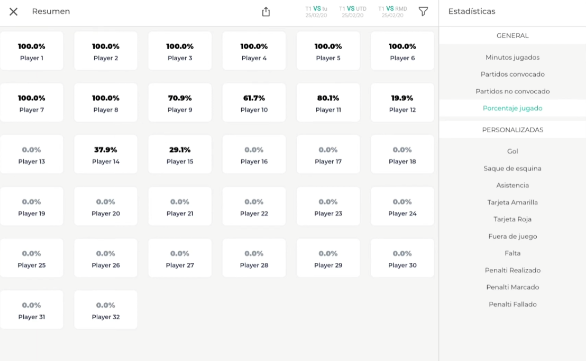
\includegraphics[width=10cm]{archivos/tfg_jorge/bcoach_ests_jugadores}
    \caption{Bcoach - Estadísticas de Jugadores}\label{sistemass2}
\end{figure}

\subsubsection{Manejo de estadísticas e indicadores de rendimiento}
Bcoach nos ofrece categorías de tarea, que se relacionarían directamente con los indicadores de rendimiento que estamos buscando. Además, ofrece estadísticas que irán siendo modificadas durante los partidos, que serán de uso para analizar esas categorías de tarea.

\begin{figure}[H]
    \centering
    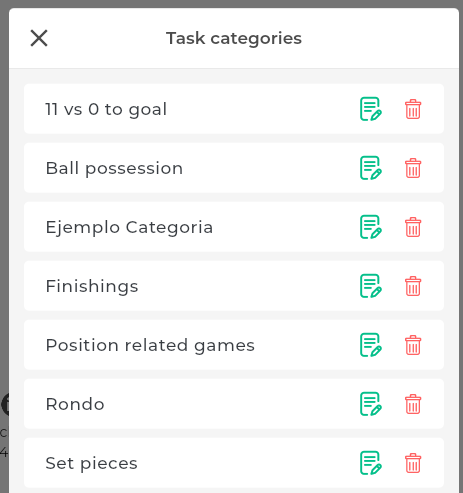
\includegraphics[width=10cm]{archivos/tfg_jorge/bcoach_kpis}
    \caption{Bcoach - Crear categoría de tarea}\label{sistemass2}
\end{figure}

\subsection{Football tactical Board}
Aplicación web gratuita con una gran variedad de deportes. Para fútbol, ofrece tres tipos de vista (Horizontal, Vertical y Medio campo). Ofrece únicamente una pizarra con figuras gráficas con la posibilidad de crear una ‘conferencia’ dónde es posible alojar a muchos usuarios que verán al mismo tiempo lo que está sucediendo en la pizarra.
Dispone de una versión Pro que elimina los anuncios y permite descargar y grabar las acciones con la pizarra.

\subsubsection{Manejo de estadísticas e indicadores de rendimiento}
Football Tactical Board es una herramienta principalmente enfocada en la creación de diagramas tácticos y la visualización de estrategias de juego. No está diseñada específicamente para la gestión y análisis de estadísticas avanzadas como los KPIs. Las funcionalidades ya nombradas permiten hacerse durante una conferencia en tiempo real, sin embargo, no aparece la opción sobre la creación de métricas.

\begin{figure}[H]
    \centering
    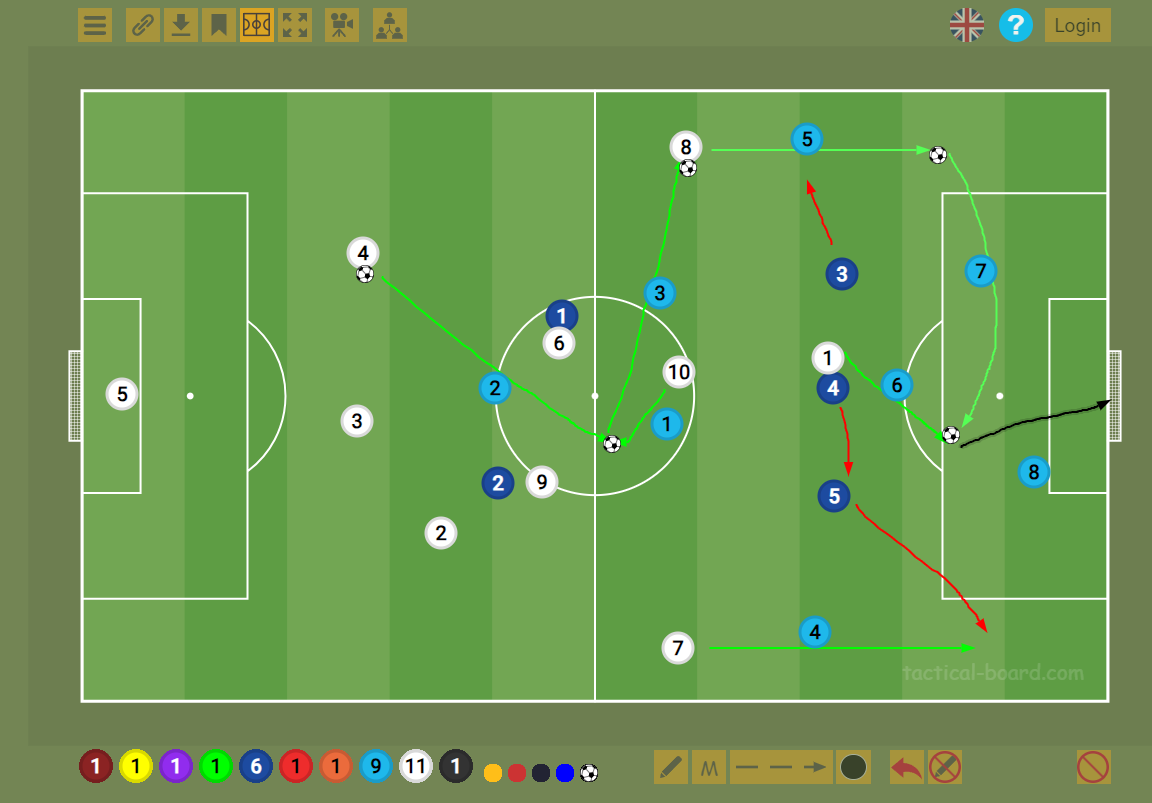
\includegraphics[width=10cm]{archivos/tfg_jorge/tbo_pizarra}
    \caption{Football Tactical Board - Pantalla del entrenador}\label{sistemass2}
\end{figure}


\subsection{Sportlyzer Players App}
Aplicación disponible tanto para Android como para IOS que ofrece opciones para entrenadores, clubes y padres

\subsubsection{Entrenadores}

\subparagraph{Horarios y Tareas}
Dispone de un calendario compartido entre todos los usuarios, cuándo el entrenador actualiza el calendario con un nuevo evento, todo el mundo podrá ver los cambios. El calendario ofrece las siguientes acciones:

\begin{itemize}
    \item Importar partidos y competiciones desde Excel
    \item Configurar entrenamientos regulares
    \item Compartir eventos por email
    \item Widget para mostrar el calendario en la web del club
    \item Anotar asistencia de los deportistas
    \item Asignación y seguimiento de deberes
\end{itemize}

\subparagraph{Disponibilidad}
Esta opción se usa para planificar actividades que necesitan mínimo de personas. Recoge información sobre qué deportistas asistirán o no a cada evento del calendario. Los enlaces son únicos para cada deportista, por lo que no necesitarán registrarse.

\subparagraph{Asistencia}
Anota la asistencia de los deportistas, pudiendo ser evaluada en un registro con el total de ausencias de cada uno, la anotación se puede hacer de forma offline.

\subparagraph{Retroalimentación}
Forma en la que los jugadores pueden comentar y valorar cada sesión, pueden dar una nota al entrenamiento, valorar cuán duro ha sido o simplemente dejar un comentario.

\subparagraph{Planificación y análisis}
Para ir desarrollando a los jugadores, la plataforma permite crear ciclos con planes de entrenamiento, pudiendo calibrar su intensidad. Después de cada uno se podrá recoger los comentarios y un análisis de los resultados.

\subparagraph{Evaluación y prueba de jugadores}
Seguimiento de cada jugador, evaluación de cada aptitud (física, táctica o técnica), personalidad y habilidades. Se puede enviar un informe de la evaluación a cada jugador. 

\subparagraph{Mensajería}
Permite enviar SMS o correos electrónicos a cada jugador y mantener conversaciones


\subsubsection{Clubes}

\subparagraph{Base de datos}
Es la manera para gestionar todos los miembros del club, en la base de datos se incluyen perfiles para deportistas, que rellenando un formulario de inscripción se crearán sus perfiles.

\subparagraph{Horarios y deberes de equipo}
Los clubes también pueden ver el calendario compartido por el entrenador y los jugadores.

\subparagraph{Facturas}
Enviar facturas a todo el club y hacer un seguimiento de los pagos, pudiendo enviar recordatorios a los impagados.

\subparagraph{Padres y Jugadores}
Este grupo de usuarios dispondrá de una app móvil donde tendrán acceso al horario de entrenamiento; mensajería con el entrenador; historial de asistencia; organizar desplazamientos a otros pares/jugadores y actualizar los detalles de contacto del jugador.


\subsubsection{Precios}
La aplicación ofrece precios mensuales o anuales (con un 30\% de descuento sobre el mensual) dependiendo del tamaño del club. La diferencia de precios escala con una diferencia de 7€ entre los tramos que van en grupos de 25 jugadores.

\subsubsection{Manejo de estadísticas e indicadores de rendimiento}
Aunque esta aplicación se enfoca en la gestión y mejora del rendimiento deportivo de los jugadores, ofrece algunas funcionalidades que pueden ser útiles para el análisis de indicadores de rendimiento. Pudiendo servir para su análisis, no se menciona en su documentación ni aparece de forma clara dentro de las interfaces ninguna opción para crear estos indicadores.

La aplicación ofrece precios mensuales o anuales (con un 30\% de descuento sobre el mensual) dependiendo del tamaño del club. La diferencia de precios escala con una diferencia de 7€ entre los tramos que van en grupos de 25 jugadores.

\begin{figure}[h]
    \centering
    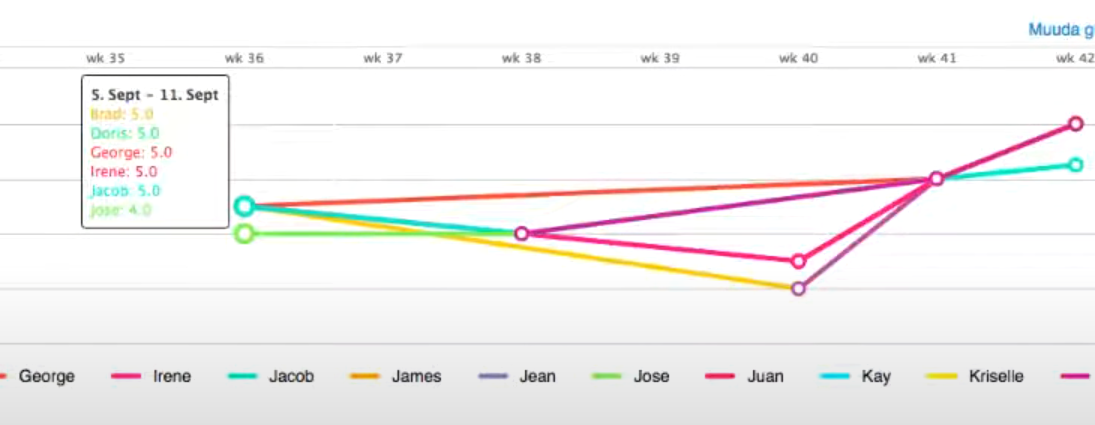
\includegraphics[width=10cm]{archivos/tfg_jorge/sportlyzer_graph_sesion_entrenamiento}
    \caption{Sportlyzer Players App - Gráfico de los tiempos de finalización del entrenamiento}\label{sistemass2}
\end{figure}


\subsection{LongoMatch}
Esta aplicación ofrece la retransmisión de partidos repetidos, con la posibilidad de dibujar sobre las imágenes de vídeo y colocar momentos importantes para ser analizados.
Ofrece dos planes diferentes:

\begin{itemize}
    \item 15€/mes o 150€/año: Proyectos ilimitados, equipos, paneles y eventos. Análisis en directo con múltiples cámaras y  administrador de base de datos.
    \item 55€/mes o 550€/año: Ofrece las posibilidades anteriores, junto con zoom durante el video, importar o exportar archivos XML y compatibilidad con otras herramientas.
\end{itemize}

\subsubsection{Manejo de estadísticas e indicadores de rendimiento}
Aunque LongoMatch no está específicamente diseñado para la creación de KPIs personalizados, se pueden crear plantillas de etiquetado que correspondan a los KPIs específicos que deseemos rastrear. Por ejemplo, puedes tener etiquetas para "Controles de Balón Exitosos", "Intercepciones", etc. Además, los informes generados por LongoMatch pueden incluir gráficos y estadísticas basadas en los eventos etiquetados, permitiendo una evaluación detallada de los KPIs.

\begin{figure}[H]
    \centering
    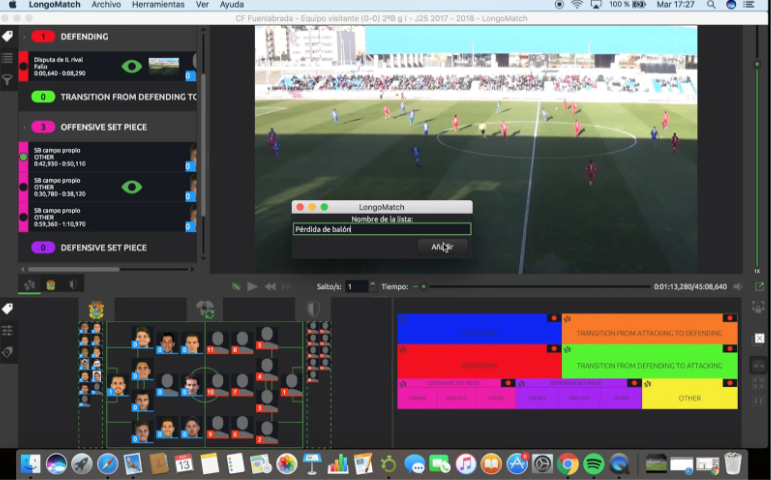
\includegraphics[width=10cm]{archivos/tfg_jorge/longomatch_eventos_live_video}
    \caption{Longomatch - Creación de eventos en el vídeo}\label{sistemass2}
\end{figure}

\subsection{Picco: Estadísticas y rendimiento}
Esta app es completamente gratis (con opción a pago para quitar anuncios) contiene una multitud de opciones para la recogida y el análisis de los datos. Durante el partido, el analista puede apuntar cada dato estadístico que él considere.
Esta pantalla de datos puede ser la más útil a la hora de recoger datos durante el partido, pues solo hay que  marcar cada registro a la vez que se va desarrollando el partido.

\subsubsection{Manejo de estadísticas e indicadores de rendimiento}
Picco es especialmente útil para la creación y seguimiento de KPIs debido a su capacidad de personalización y análisis detallado. Tiene la posibilidad de definir KPIs específicos , por ejemplo, puedes crear indicadores como "Tasa de éxito en pases", "Distancia recorrida por jugador", entre otros. Todos estos siendo recogidos y actualizados en tiempo real asegurando datos precisos y disponibilidad inmediata.

\begin{figure}[H]
    \centering
    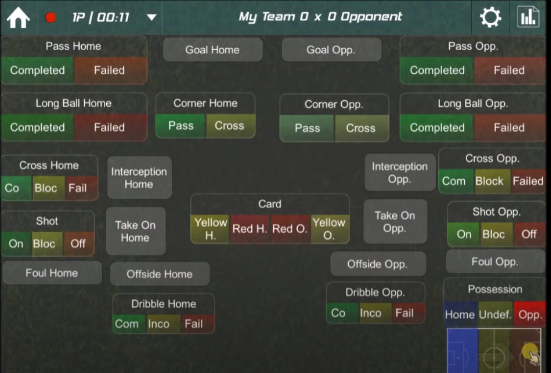
\includegraphics[width=10cm]{archivos/tfg_jorge/picco_ui_partidos}
    \caption{Picco - Interfaz durante el partido}\label{sistemass2}
\end{figure}

\subsection{Teamtag}
Esta aplicación es parecida a la Picco, teniendo funcionalidades más allá de los pocos paneles que contiene Picco, esta aplicación se enfoca en la gestión de un club, pudiendo crear eventos de partidos para ir apuntando las estadísticas a medida que transcurre el evento. Permite crear tus propios equipos y alineaciones para cuando un evento estadístico sea registrado, indicar que jugador/a lo ocasionó y en qué zona del campo ocurrió.

\subsubsection{Manejo de estadísticas e indicadores de rendimiento}
Al igual que la aplicación anterior, permite la definición de indicadores personalizados que se irán recogiendo en tiempo real.

\begin{figure}[H]
    \centering
    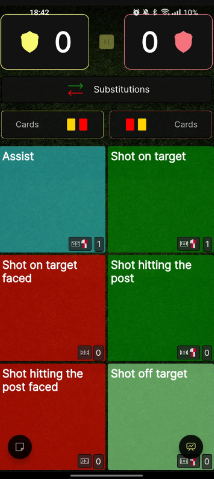
\includegraphics[width=3cm]{archivos/tfg_jorge/teamtag_movil_ui}
    \caption{Teamtag - Interfaz durante el partido}\label{sistemass2}
\end{figure}

\subsection{Conclusiones}
Una vez analizadas las aplicaciones del mercado, podemos concluir la función de cada una.
Bcoach:
\begin{itemize}
    \item Planificación de entrenamientos con animaciones.
    \item Pizarra táctica.
    \item Estadísticas de partidos.
    \item Planes desde 2,99€/mes.
\end{itemize}

Sportlyzer Players App:
\begin{itemize}
    \item Para entrenadores, clubes y jugadores.
    \item Horarios y tareas con calendario compartido.
    \item Asignación de deberes y seguimiento de asistencia.
    \item Evaluación y análisis de jugadores.
    \item Mensajería con jugadores.
    \item Planes desde 7€/mes por jugador.
\end{itemize}

LongoMatch:
\begin{itemize}
    \item Retransmisión de partidos repetidos.
    \item Dibujar sobre video y análisis de momentos importantes.
    \item Planes desde 15€/mes.
\end{itemize}

Picco y Teamtag:
\begin{itemize}
    \item Recogida y análisis de datos estadísticos.
    \item Gratis (con opción de pago para quitar anuncios).
\end{itemize}

Dependiendo de las necesidades, Bcoach o Sportlyzer podrían ser las más completas para la gestión de los equipos. Y si el problema es el presupuesto, Football Tactical Board o Picco podrían ser también buenas opciones

\subsubsection{Manejo de estadísticas e indicadores de rendimiento}
El manejo de estadísticas e indicadores de rendimiento es crucial para el análisis y la mejora continua del desempeño de los jugadores y equipos. Cada una de las aplicaciones analizadas ofrece diferentes niveles de soporte para estas funcionalidades:

\subparagraph{Bcoach}
\begin{itemize}
    \item Ofrece categorías de tarea que se relacionan directamente con los indicadores de rendimiento.
    \item Estadísticas que se modifican durante los partidos para analizar esas categorías.
\end{itemize}
\subparagraph{Football Tactical Board}
\begin{itemize}
    \item Enfocada en la creación de diagramas tácticos y estrategias de juego.
    \item No diseñada específicamente para la gestión y análisis de estadísticas avanzadas como los KPIs.
\end{itemize}

\subparagraph{Sportlyzer Players App}
\begin{itemize}
    \item Enfocada en la gestión y mejora del rendimiento deportivo.
    \item Funcionalidades útiles para el análisis de indicadores de rendimiento, aunque no ofrece una opción clara para la creación de KPIs.
\end{itemize}

\subparagraph{LongoMatch}
\begin{itemize}
    \item Permite etiquetar eventos específicos durante los partidos y analizarlos posteriormente.
    \item Informes generados pueden incluir gráficos y estadísticas basadas en los eventos etiquetados.
\end{itemize}

\subparagraph{Picco}
\begin{itemize}
    \item Especialmente útil para la creación y seguimiento de KPIs debido a su capacidad de personalización.
    \item Recogida y actualización de datos en tiempo real.
\end{itemize}

\subparagraph{Teamtag}
\begin{itemize}
    \item Permite la definición de indicadores personalizados que se irán recogiendo en tiempo real.
    \item Gestión de equipos y alineaciones, registro de eventos y análisis de datos.
\end{itemize}

En resumen, todas las aplicaciones analizadas ofrecen herramientas útiles para el manejo de estadísticas e indicadores de rendimiento, aunque no todas ofrecen la opción de crear indicadores personalizados.
\section{Tabla comparativa}

\begin{table}[ht]
{\tiny % Usar \tiny o \scriptsize para hacerlo aún más pequeño
\begin{tabular}{|m{14mm}|m{12mm}|m{14mm}|m{10mm}|m{14mm}|m{8mm}|m{14mm}|m{12mm}|m{10mm}|m{14mm}|}
\hline
\textbf{Aplicación} & \textbf{Estadísticas predefinidas} & \textbf{Creación de nuevas estadísticas} & \textbf{En tiempo real} & \textbf{Individuales} & \textbf{Grupales} & \textbf{Informe generado} & \textbf{Seguimiento contínuo} & \textbf{Toma de decisión} & \textbf{KPIs Personalizables} \\
\hline
Bcoach & \ding{51} & \ding{51} & \ding{51} & \ding{51} & \ding{51} & \ding{51} & \ding{51} & \ding{55} & \ding{51} \\
\hline
Sportlyzer Players App & \ding{51} & \ding{55} & \ding{55} & \ding{51} & \ding{51} & \ding{51} & \ding{51} & \ding{55} & \ding{55} \\
\hline
LongoMatch & \ding{55} & \ding{51} & \ding{51} & \ding{55} & \ding{51} & \ding{55} & \ding{55} & \ding{55} & \ding{55} \\
\hline
Picco & \ding{51} & \ding{51} & \ding{51} & \ding{55} & \ding{51} & \ding{55} & \ding{55} & \ding{55} & \ding{51} \\
\hline
Teamtag & \ding{51} & \ding{55} & \ding{51} & \ding{51} & \ding{51} & \ding{51} & \ding{51} & \ding{55} & \ding{51} \\
\hline
\end{tabular}
\caption{Comparativa de funcionalidades de aplicaciones} % Título de la tabla para el índice y visualización
\label{tab:comparativa_funcionalidades} % Etiqueta para referencias cruzadas
}
\end{table}

	% Plantilla: Se muestran listas
%%%%%%%%%%%%%%%%%%%%%%%%%%%%%%%%%%%%%%%%%%%%%%%%%%%%%%%%%%%%%%%%%%%%%%%%
% Plantilla TFG/TFM
% Escuela Politécnica Superior de la Universidad de Alicante
% Realizado por: Jose Manuel Requena Plens
% Contacto: info@jmrplens.com / Telegram:@jmrplens
%%%%%%%%%%%%%%%%%%%%%%%%%%%%%%%%%%%%%%%%%%%%%%%%%%%%%%%%%%%%%%%%%%%%%%%%

\chapter{Objetivos}
\label{objetivos}

\section{Objetivos generales}
La plataforma va dirigida a todos los entrenadores/as de divisiones inferiores con el fin de agilizar y conseguir de la manera más eficaz y eficiente posible el correcto desarrollo de los jugadores.

Siguiendo las definiciones de la doctora Deborah Hoare en [\cite{DHoare}], después de identificar y seleccionar talentos, es imperativo poner a disposición del deportista una infraestructura adecuada que les permita desarrollar su potencial al máximo. Esto implica no solo un buen programa de entrenamiento y competición bien estructurado, sino también el acceso al equipo necesario para su competencia.

La plataforma facilita este acceso proporcionando un sistema integrado que ayuda a los entrenadores a planificar y ejecutar programas de entrenamiento adaptados a las necesidades individuales o grupales de cada jugador. También permitirá un seguimiento detallado del progreso del equipo, garantizando maximizar sus resultados y que se identifican áreas de mejora comprendidas en una matriz DAFO (Debilidades, Amenazas, Fortalezas y Oportunidades).

Se busca la optimización del proceso de evaluación, implementado herramientas automatizadas que permitan a los entrenadores realizar análisis y valoraciones en tiempo real durante los entrenamientos y partidos. Los datos podrán serán capturados mediando dispositivos que el usuario lleve consigo o a través de aplicaciones móviles.
Los datos recogidos se utilizarán para elaborar análisis históricos de los jugadores para predecir tendencias. Esto ayudará a los entrenadores a tomar decisiones correctas sobre la carga de entrenamiento y la rotación del equipo para optimizar el rendimiento.

En resumen, la plataforma busca ser una herramienta esencial en el arsenal de cualquier entrenador que trabaje con jóvenes jugadores, proporcionándoles las capacidades necesarias para fomentar el desarrollo de sus capacidades en el fútbol y otros deportes. Con esta herramienta, los entrenadores pueden asegurarse de que cada jugador no solo alcanza su potencial técnico y táctico, sino que también recibe el soporte físico y psicológico necesario para su desarrollo integral.

\section{Objetivos específicos}
\begin{enumerate}
    \item \textbf{Identificación y desarrollo del talento:}
    \begin{itemize}
        \item Descripción de la infraestructura adecuada y programas de entrenamiento.
    \end{itemize}

    \item \textbf{Acceso a herramientas y equipo necesario:}
    \begin{itemize}
        \item Planificación y ejecución de programas de entrenamiento adaptados a las necesidades individuales y grupales.
    \end{itemize}

    \item \textbf{Seguimiento y evaluación del progreso:}
    \begin{itemize}
        \item Uso de herramientas automatizadas para el análisis en tiempo real durante entrenamientos y partidos.
    \end{itemize}

    \item \textbf{Análisis histórico y predicción de tendencias:}
    \begin{itemize}
        \item Utilización de datos históricos para optimizar la carga de entrenamiento y la rotación del equipo.
    \end{itemize}
\end{enumerate}
		% Plantilla: Se muestran tablas
%%%%%%%%%%%%%%%%%%%%%%%%%%%%%%%%%%%%%%%%%%%%%%%%%%%%%%%%%%%%%%%%%%%%%%%%
% Plantilla TFG/TFM
% Escuela Politécnica Superior de la Universidad de Alicante
% Realizado por: Jose Manuel Requena Plens
% Contacto: info@jmrplens.com / Telegram:@jmrplens
%%%%%%%%%%%%%%%%%%%%%%%%%%%%%%%%%%%%%%%%%%%%%%%%%%%%%%%%%%%%%%%%%%%%%%%%

\chapter{Metodología}
\label{metodologia}

\section{Historias de usuario}
Para la gestión ágil de este proyecto, comenzaremos a describir historias de usuario. Siguiendo una estructura sistemática para reflejar las necesidades de los usuarios que se traducen en requisitos funcionales para el sistema que influirán en el diseño y desarrollo de la plataforma.

%-------------------------------------------------------------------
\begin{tcolorbox}[title=Historia de Usuario 1: Añadir KPIs a la pantalla de estadísticas]
\textbf{Como} \textit{Entrenador/a},\\
\textbf{Quiero} Poder añadir y quitar KPIs de la pantalla de estadísticas según sea necesario,\\
\textbf{Para que} Enfocarme en medir y visualizar solo los KPIs específicos que necesito, facilitando la toma de decisiones rápidas y efectivas para mejorar el rendimiento del equipo.
\end{tcolorbox}

\subparagraph{Descripción}
La pantalla para evaluar los indicadores de rendimiento debe mostrar a la vez tantos como el entrenador necesite al mismo tiempo, así como eliminar de la vista aquellos que ya no son relevantes en ese momento.

\subparagraph{Criterios de Aceptación}
\begin{itemize}
    \item El entrenador debe poder acceder a una interfaz de usuario para ver los KPIs.
    \item La aplicación debe recomendar algunos KPIs predefinidos en caso de que haya menos de 5 en la pantalla.
    \item El entrenador debe poder borrar todos los indicadores de una sola vez y limpiar la vista.
\end{itemize}

%-------------------------------------------------------------------
\begin{tcolorbox}[title=Historia de Usuario 2: Creación de nuevos KPIs]
\textbf{Como} \textit{Entrenador/a},\\
\textbf{Quiero} Poder crear y eliminar nuevos indicadores de rendimiento con los datos almacenados en la base de datos,\\
\textbf{Para que} Explotar todos los datos recopilados de una manera eficiente para ver las fortalezas y debilidades del equipo.
\end{tcolorbox}

\subparagraph{Descripción}
Después de cada partido o entrenamiento, los datos comunicados por el entrenador serán almacenados en una base de datos. A partir de esos datos y con una fórmula general, el entrenador debe poder elegir dos datos y crear un nuevo indicador de rendimiento para ser evaluado.

\subparagraph{Criterios de Aceptación}
\begin{itemize}
    \item El entrenador debe poder acceder a una interfaz de usuario para crear los KPIs.
    \item En la interfaz se debe poder definir el nuevo nombre del indicador, descripción y los datos que involucra.
    \item La aplicación no debe permitir nombres repetidos de indicadores.
    \item La aplicación no debe permitir que dos indicadores involucren los mismos datos de la misma forma.
    \item El indicador debe poder asignarse a jugadores o equipos.
\end{itemize}

%-------------------------------------------------------------------
\begin{tcolorbox}[title=Historia de Usuario 3: Edición de KPIs]
\textbf{Como} \textit{Entrenador/a},\\
\textbf{Quiero} Poder editar los indicadores de rendimiento ya sea por su nombre o por sus parámetros,\\
\textbf{Para que} Cambiar los indicadores según el progreso que necesiten mis entrenamientos.
\end{tcolorbox}

\subparagraph{Descripción}
Una vez haya definido al menos un KPI, el entrenador debe ser capaz de editar el nombre, atributos y descripción del indicador. Este cambio puede ser debido ya sea por el cambio de opinión del entrenador del entrenador, o por una necesidad de utilizar ese nombre o parámetros para otra perspectiva en las sesiones de entrenamiento.

\subparagraph{Criterios de Aceptación}
\begin{itemize}
    \item El entrenador debe poder seleccionar un KPI existente en la interfaz para editarlo.
    \item La interfaz de edición debe poder permitir editar el nombre, parámetros del KPI o jugadores y equipo a los cuales esté asignado este indicador.
    \item Los cambios deben de ser en cascada, reflejando la modificación en todas las vistas en las que el KPI esté implicado.
    \item Se debe permitir cancelar la edición si el usuario cambia de idea.
\end{itemize}

%-------------------------------------------------------------------
\begin{tcolorbox}[title=Historia de Usuario 4: Ver estadísticas]
\textbf{Como} \textit{Jugador/a},\\
\textbf{Quiero} Poder ver un listado de todas mis estadísticas y mis indicadores de rendimiento,\\
\textbf{Para que} Poder fijarme en mis puntos débiles e intentar mejorarlos según me dicte el entrenador.
\end{tcolorbox}

\subparagraph{Descripción}
Cada jugador debe poder acceder a una interfaz donde se muestren todos los indicadores que el entrenador ha asociado a ese jugador en concreto, también debería ver una gráfica sobre el progreso y la evolución de sus indicadores. Así se podría fomentar la auto-crítica por parte del jugador.

\subparagraph{Criterios de Aceptación}
\begin{itemize}
    \item Los jugadores deben poder acceder a un menú propio donde se muestren sus datos.
    \item El menú debe incluir gráficas con marcas temporales.
    \item Se de poder filtrar por rango de fechas, seleccionar estadísticas para que solo se muestren esas y por tipos de estadísticas.
\end{itemize}

%-------------------------------------------------------------------
\begin{tcolorbox}[title=Historia de Usuario 5: Ver progreso de los jugadores]
\textbf{Como} \textit{Entrenador/a},\\
\textbf{Quiero} Poder generar un informe gráfico que muestre la evolución de los KPIs asociados a jugadores,\\
\textbf{Para que} Poder evaluar a mis jugadores y darles las indicaciones adecuadas para maximizar el margen de mejora de mi equipo.
\end{tcolorbox}

\subparagraph{Descripción}
El entrenador es el primer responsable del equipo y de él depende que los jugadores mejoren y exploten sus capacidades lo máximo posible. Es por ello que debe de ser capaz de generar en la plataforma un informe, ya sea individual de cada jugador o grupal, sobre la evolución de las estadísticas de éstos.

\subparagraph{Criterios de Aceptación}
\begin{itemize}
    \item Los entrenadores deben poder seleccionar uno o varios jugadores junto con uno o varios KPIs para generar el informe.
    \item El menú debe incluir gráficas con marcas temporales.
    \item La plataforma debe de ser capaz de detectar una mejora o un empeoramiento de las habilidades del jugador.
\end{itemize}


%-------------------------------------------------------------------
\begin{tcolorbox}[title=Historia de Usuario 6: Alinear jugadores del Equipo]
\textbf{Como} \textit{Entrenador/a},\\
\textbf{Quiero} Poder crear nuevas alineaciones con mis jugadores del equipo,\\
\textbf{Para que} Plantear tácticas, posicionar jugadores y descubrir y fortalecer las buenas posiciones para mis jugadores.
\end{tcolorbox}

\subparagraph{Descripción}
Entender las posiciones de los jugadores es una tarea clave para el entrenador, por ello ha de ser capaz de poder crear nuevas alineaciones con sus jugadores para poder entenderlos a la perfección.

\subparagraph{Criterios de Aceptación}
\begin{itemize}
    \item Los entrenadores deben poder acceder a un menú dentro de la vista del equipo para la creación de alineaciones.
    \item Un jugador no puede aparecer dos veces en la misma alineación.
    \item En la vista de la alineación, se debe poder editar y eliminar toda la alineación.
    \item Se dispondrá de alineaciones comunes predefinidas, con la posibilidad del entrenador de crear las suyas propias.
    \item No podrán existir dos alineaciones exactamente iguales (mismos jugadores en la misma posición).
\end{itemize}

%-------------------------------------------------------------------
\begin{tcolorbox}[title=Historia de Usuario 7: Análisis y Reportes Detallados]
\textbf{Como} \textit{Entrenador/a},\\
\textbf{Quiero} Generar reportes detallados de rendimiento por jugador y por equipo,\\
\textbf{Para que} Tener un seguimiento preciso del progreso a lo largo del tiempo.
\end{tcolorbox}

\subparagraph{Descripción}
Más allá de un visualizado de estadísticas y gráficas, el entrenador debe se capaz de generar informes completos sobre el desarrollo de los jugadores.

\subparagraph{Criterios de Aceptación}
\begin{itemize}
    \item Para generar los informes, se debe poder seleccionar métricas específicas.
    \item Los informes pueden ser exportados en formatos PDF, Excel o CSV.
    \item Los informes deben contener gráficas de tendencias y otras comparativas.
\end{itemize}

%-------------------------------------------------------------------
\begin{tcolorbox}[title=Historia de Usuario 8: Sistema de comunicación]
\textbf{Como} \textit{Entrenador/a o jugador/a},\\
\textbf{Quiero} Poder comunicarme con mis jugadores/entrenador,\\
\textbf{Para que} favorecer la comunicación y mejorar el ambiente del equipo.
\end{tcolorbox}

\subparagraph{Descripción}
Además del seguimiento de estadísticas, si ocurren acontecimientos que requieran de una conversación entre el entrenador y el jugador se debería contar con un sistema simple de mensajería. Con este pequeño sistema dentro de la plataforma, es posible fomentar un ambiente de equipo positivo siguiendo las palabras de Sir Alex Ferguson en \cite{TheGuardian} .

\subparagraph{Criterios de Aceptación}
\begin{itemize}
    \item Debe de exisitr una interfaz dedicada a la mensajería.
    \item Las conversaciones permanecerán almacenadas hasta que el usuario decida borrarlas.
    \item Se debe poder iniciar y borrar conversaciones desde un menú.
    \item No podrán existir dos chats con la misma persona.
\end{itemize}


%-------------------------------------------------------------------
\begin{tcolorbox}[title=Historia de Usuario 9: Acceso a roles de usuario]
\textbf{Como} \textit{Usuario},\\
\textbf{Quiero} Poder acceder a los datos a los que tenga acceso,\\
\textbf{Para que} Realizar el seguimiento siendo o el mismo jugador o el tutor legal de éste.
\end{tcolorbox}

\subparagraph{Descripción}
Los padres y tutores también tienen derecho a ver el seguimiento de sus hijos/as, por ello es considerable añadir roles de usuario para que cada persona responsable pueda ver sus propios datos.

\subparagraph{Criterios de Aceptación}
\begin{itemize}
    \item La plataforma debe tener definidos claramente los roles de "Entrenador", "Jugador", "Padre/Tutor" y "Administrador".
    \item Cada rol debe poder acceder únicamente a los datos que le corresponden según las definiciones de permisos.
    \item Debe existir un sistema de autenticación para los usuarios.
    \item La plataforma debe cumplir con las normativas locales e internacionales de protección de datos
\end{itemize}

%-------------------------------------------------------------------
\begin{tcolorbox}[title=Historia de Usuario 10: Intervalos Estadísticos para el menú]
\textbf{Como} \textit{Entrenador/a},\\
\textbf{Quiero} Poder alternar el intervalo de tiempo en el que se mide la estadística,\\
\textbf{Para que} Tener un mejor control de la evolución de mis equipos durante el periodo de tiempo que estime útil.
\end{tcolorbox}

\subparagraph{Descripción}
Para que el seguimiento de los resultados sea lo mas eficaz y eficiente posible, el entrenador debe poder alternar el intervalo de tiempo en el que se miden los resultados para su propio interés. Si quiere ver resultados a corto plazo, podrá ver la evolución partido a partido, si quiere resultados a largo plazo, oidrá verla mensual o trimestralmente.

\subparagraph{Criterios de Aceptación}
\begin{itemize}
    \item La plataforma tendrá un menú superior para alternar el intervalo.
    \item Cuando se alterna la opción, todas las vistas serán actualizadas para mostrar la evolución de los jugadores dentro del intervalo seleccionado.
\end{itemize}

%Para Añadir:
%- Creación de secciones para los KPIs
%- Intervalos Estadísticos para el menú
%- DAFO para la ficha de jugadores

\section{Elección de las tecnologías y lenguajes de programación}
A continuación, detallamos las razones específicas para la elección de las siguientes herramientas como componentes clave del desarrollo.

\subsection{Git}

\subsection{Visual Studio Code}


\subsection{VueJS}

\subsubsection{Dependencias}


\subsection{MySQL Server}

\subsection{Framework DAO}
Cambiar en database.js \lstinline|require("mysql")| por \lstinline|mysql2|, compatible con el método \lstinline|auth_caching_sha2_password|, el que viene en MySQL Server 8.4.

	% Plantilla: Se muestran figuras
%%%%%%%%%%%%%%%%%%%%%%%%%%%%%%%%%%%%%%%%%%%%%%%%%%%%%%%%%%%%%%%%%%%%%%%%
% Plantilla TFG/TFM
% Escuela Politécnica Superior de la Universidad de Alicante
% Realizado por: Jose Manuel Requena Plens
% Contacto: info@jmrplens.com / Telegram:@jmrplens
%%%%%%%%%%%%%%%%%%%%%%%%%%%%%%%%%%%%%%%%%%%%%%%%%%%%%%%%%%%%%%%%%%%%%%%%

\chapter{Desarrollo}
\label{desarrollo}
\section{Requisitos}
En esta sección realizaremos una toma de los requisitos generales del sistema, seguidos de requisitos específicos.
\subsection{Funcionales}
Los requisitos funcionales son especificaciones que definen las funciones o características que un sistema debe poseer. Estos describen el comportamiento del sistema bajo ciertas condiciones y definen lo que el sistema debe hacer.

\subsubsection{Generales}
\begin{itemize}
    \item \textbf{R1:} Cada uno de los usuarios tendrá acceso a una información específica, pudiendo acceder solamente a los datos y funciones a los que tenga permiso ver.
    
    \item \textbf{R2:} Cada uno de los usuarios tendrá acceso a una información específica, pudiendo acceder solamente a los datos y funciones a los que tenga permiso ver.
    
    \item \textbf{R3:} Se podrán generar informes de rendimiento para los jugadores y el equipo técnico.
    
    \item \textbf{R4:} Cada entrenador de una organización podrá acceder a la información de todos los actores que forman parte de la organización.
    
    \item \textbf{R5:} Los entrenadores tendrán acceso a todas las sesiones de entrenamiento y a estadísticas individuales y grupales de cada jugador.    
\end{itemize}

\subsubsection{Entrenamientos}
\begin{itemize}
    \item \textbf{R6:} Los usuarios tendrán un apartado para acceder a un calendario, que mostrará cada sesión.
    \item \textbf{R7:} Para cada sesión, se mostará específicamente el nombre de ésta, el dia y la hora de inicio y fin de la sesión.
    
\end{itemize}

\subsubsection{Seguimiento y Evaluación del Rendimiento}
\begin{itemize}
    \item \textbf{R8:} Evaluar el rendimiento de los jugadores mediante la recolección de estadísticas durante los entrenamientos y partidos.
    
    \item \textbf{R9:} Mostrar el historial de puntuaciones dadas por el entrenador por cada intervalo de  tiempo definido.
    
    \item \textbf{R9:} Elaborar gráficos de las puntuaciones de los KPIs para todo el equipo para que se pueda apreciar la evolución del equipo en un conjunto.
    
    \item \textbf{R10:} Elaborar gráficos de las puntuaciones de los KPIs para cada jugador, pudiendo apreciarse la evolución individual.
    
    \item \textbf{R11:} Desarrollar un algoritmo estadístico para generar una matriz DAFO (debilidades, Amenazas, Fortalezas y Debilidades) que permitan al entrenador analizar de una manera más precisa las necesidades de sus jugadores.
    
\end{itemize}

\subsubsection{Equipo}
\begin{itemize}
    \item \textbf{R12:} El entrenador podrá ver toda la información detallada del equipo
    
    \item \textbf{R13:} El entrenador podrá ver toda la información detallada de cada jugador individualmente
    
\end{itemize}

\subsubsection{Intervalos de tiempo}
\begin{itemize}
    \item \textbf{R14:} Los usuarios podrán acceder a un histórico de los datos en un intervalo de tiempo correspondiente a una sesión.
    
    \item \textbf{R15:} Los usuarios podrán acceder a un histórico de los datos en un intervalo de tiempo correspondiente a un mes.
    
    \item \textbf{R16:} Los usuarios podrán acceder a un histórico de los datos en un intervalo de tiempo correspondiente a un trimestre.
    
\end{itemize}

\subsubsection{Actores}
\begin{itemize}
    \item \textbf{R17:} Los entrenadores podrán acceder a la información de los actores que componen la organización y sean jugadores.
    
    \item \textbf{R18:} Cada ventana del actor tendrá su información correspondiente al seguimiento de dicho actor.
    
\end{itemize}

\subsection{No Funcionales}
Los requisitos no funcionales describen cómo el sistema debe comportarse. Estos incluyen aspectos como el rendimiento, la seguridad, la usabilidad, la escalabilidad y la disponibilidad del sistema.

\subsubsection{Rendimiento}
\begin{itemize}
    \item \textbf{Capacidad de carga:} La plataforma debe ser capaz de manejar una cantidad considerable de usuarios simultáneos sin afectar al rendimiento.
    
    \item \textbf{Tiempo de Respuesta:} La carga de los datos debe completarse en un tiempo rápido.
    
    \item \textbf{Optimización:} Las consultas a la base de datos deben de estar optimizadas para minimizar el tiempo de espera.
    
\end{itemize}

\subsubsection{Seguridad}
\begin{itemize}
    \item \textbf{Autenticación:} Las operaciones de carga de datos no se realizarán hasta que el usuario no se haya autenticado correctamente.
    
    \item \textbf{Protección de datos:} Los datos personales de los usuarios deben ser almacenados y procesados conforme a las normativas de protección de datos.
    
\end{itemize}

\subsubsection{Usabilidad}
\begin{itemize}
    \item \textbf{Interfaz intuitiva:} La interfaz de usuario debe ser intuitiva y fácil de usar, permitiendo a los usuarios utilizar la plataforma desde cero sin tener que formarse para ello.
    
    \item \textbf{Documentación:} Los usuarios deben poder acceder a una documentación clara para usar la plataforma.
    
\end{itemize}

\subsubsection{Escalabilidad}
\begin{itemize}
    \item \textbf{Escalabilidad horizontal:} La plataforma debe poder escalar horizontalmente (añadiendo mas servidores) para reducir la carga de éstos y mejorar la experiencia del usuario.
    
    \item \textbf{Escalabilidad vertical:} La plataforma debe poder escalar verticalmente (mejorando los servidores) para manejar el aumento de usuarios y la carga de trabajo.
    
\end{itemize}

\subsubsection{Compatibilidad}
\begin{itemize}
    \item \textbf{Multiplataforma:} La plataforma ser accesible en distintos sistemas operativos, así como desde diferentes tipos de dispositivo (móvil u ordenadores).
    
\end{itemize}

\subsubsection{Fiabilidad}
\begin{itemize}
    \item \textbf{Tolerancia a fallos:} El sistema debe manejar los errores de una manera adecuada, proporcionando mensajes de error claros para su rápida resolución.
    
    \item \textbf{Consistencia de datos:} Los datos deben mantenerse consistentes y libres de errores.
    
\end{itemize}

\section{Análisis funcional del sistema}

\subsection{Historias de usuario}

Para la gestión ágil de este proyecto, comenzaremos a describir historias de usuario. Siguiendo una estructura sistemática para reflejar las necesidades de los usuarios que se traducen en requisitos funcionales para el sistema que influirán en el diseño y desarrollo de la plataforma.

%-------------------------------------------------------------------
\begin{tcolorbox}[title= Añadir KPIs a la pantalla de estadísticas]
\textbf{Como} \textit{Entrenador/a},\\
\textbf{Quiero} Poder añadir y quitar KPIs de la pantalla de estadísticas según sea necesario,\\
\textbf{Para que} Enfocarme en medir y visualizar solo los KPIs específicos que necesito, facilitando la toma de decisiones rápidas y efectivas para mejorar el rendimiento del equipo.
\end{tcolorbox}

\subparagraph{Descripción}
La pantalla para evaluar los indicadores de rendimiento debe mostrar a la vez tantos como el entrenador necesite al mismo tiempo, así como eliminar de la vista aquellos que ya no son relevantes en ese momento.

\subparagraph{Criterios de Aceptación}
\begin{itemize}
    \item El entrenador debe poder acceder a una interfaz de usuario para ver los KPIs.
    \item La aplicación debe recomendar algunos KPIs predefinidos en caso de que haya menos de 5 en la pantalla.
    \item El entrenador debe poder borrar todos los indicadores de una sola vez y limpiar la vista.
\end{itemize}

%-------------------------------------------------------------------
\begin{tcolorbox}[title=Creación de nuevos KPIs]
\textbf{Como} \textit{Entrenador/a},\\
\textbf{Quiero} Poder crear y eliminar nuevos indicadores de rendimiento con los datos almacenados en la base de datos,\\
\textbf{Para que} Explotar todos los datos recopilados de una manera eficiente para ver las fortalezas y debilidades del equipo.
\end{tcolorbox}

\subparagraph{Descripción}
Después de cada partido o entrenamiento, los datos comunicados por el entrenador serán almacenados en una base de datos. A partir de esos datos y con una fórmula general, el entrenador debe poder elegir dos datos y crear un nuevo indicador de rendimiento para ser evaluado.

\subparagraph{Criterios de Aceptación}
\begin{itemize}
    \item El entrenador debe poder acceder a una interfaz de usuario para crear los KPIs.
    \item En la interfaz se debe poder definir el nuevo nombre del indicador, descripción y los datos que involucra.
    \item La aplicación no debe permitir nombres repetidos de indicadores.
    \item La aplicación no debe permitir que dos indicadores involucren los mismos datos de la misma forma.
    \item El indicador debe poder asignarse a jugadores o equipos.
\end{itemize}

%-------------------------------------------------------------------
\begin{tcolorbox}[title=Edición de KPIs]
\textbf{Como} \textit{Entrenador/a},\\
\textbf{Quiero} Poder editar los indicadores de rendimiento ya sea por su nombre o por sus parámetros,\\
\textbf{Para que} Cambiar los indicadores según el progreso que necesiten mis entrenamientos.
\end{tcolorbox}

\subparagraph{Descripción}
Una vez haya definido al menos un KPI, el entrenador debe ser capaz de editar el nombre, atributos y descripción del indicador. Este cambio puede ser debido ya sea por el cambio de opinión del entrenador del entrenador, o por una necesidad de utilizar ese nombre o parámetros para otra perspectiva en las sesiones de entrenamiento.

\subparagraph{Criterios de Aceptación}
\begin{itemize}
    \item El entrenador debe poder seleccionar un KPI existente en la interfaz para editarlo.
    \item La interfaz de edición debe poder permitir editar el nombre, parámetros del KPI o jugadores y equipo a los cuales esté asignado este indicador.
    \item Los cambios deben de ser en cascada, reflejando la modificación en todas las vistas en las que el KPI esté implicado.
    \item Se debe permitir cancelar la edición si el usuario cambia de idea.
\end{itemize}

%-------------------------------------------------------------------
\begin{tcolorbox}[title=Ver estadísticas]
\textbf{Como} \textit{Jugador/a},\\
\textbf{Quiero} Poder ver un listado de todas mis estadísticas y mis indicadores de rendimiento,\\
\textbf{Para que} Poder fijarme en mis puntos débiles e intentar mejorarlos según me dicte el entrenador.
\end{tcolorbox}

\subparagraph{Descripción}
Cada jugador debe poder acceder a una interfaz donde se muestren todos los indicadores que el entrenador ha asociado a ese jugador en concreto, también debería ver una gráfica sobre el progreso y la evolución de sus indicadores. Así se podría fomentar la auto-crítica por parte del jugador.

\subparagraph{Criterios de Aceptación}
\begin{itemize}
    \item Los jugadores deben poder acceder a un menú propio donde se muestren sus datos.
    \item El menú debe incluir gráficas con marcas temporales.
    \item Se de poder filtrar por rango de fechas, seleccionar estadísticas para que solo se muestren esas y por tipos de estadísticas.
\end{itemize}

%-------------------------------------------------------------------
\begin{tcolorbox}[title=Ver progreso de los jugadores]
\textbf{Como} \textit{Entrenador/a},\\
\textbf{Quiero} Poder generar un informe gráfico que muestre la evolución de los KPIs asociados a jugadores,\\
\textbf{Para que} Poder evaluar a mis jugadores y darles las indicaciones adecuadas para maximizar el margen de mejora de mi equipo.
\end{tcolorbox}

\section{Implementación}

\subparagraph{Descripción}
El entrenador es el primer responsable del equipo y de él depende que los jugadores mejoren y exploten sus capacidades lo máximo posible. Es por ello que debe de ser capaz de generar en la plataforma un informe, ya sea individual de cada jugador o grupal, sobre la evolución de las estadísticas de éstos.

\subparagraph{Criterios de Aceptación}
\begin{itemize}
    \item Los entrenadores deben poder seleccionar uno o varios jugadores junto con uno o varios KPIs para generar el informe.
    \item El menú debe incluir gráficas con marcas temporales.
    \item La plataforma debe de ser capaz de detectar una mejora o un empeoramiento de las habilidades del jugador.
\end{itemize}


%-------------------------------------------------------------------
\begin{tcolorbox}[title=Historia de Usuario: Análisis y Reportes Detallados]
\textbf{Como} \textit{Entrenador/a},\\
\textbf{Quiero} Generar reportes detallados de rendimiento por jugador y por equipo,\\
\textbf{Para que} Tener un seguimiento preciso del progreso a lo largo del tiempo.
\end{tcolorbox}

\subparagraph{Descripción}
Más allá de un visualizado de estadísticas y gráficas, el entrenador debe se capaz de generar informes completos sobre el desarrollo de los jugadores.

\subparagraph{Criterios de Aceptación}
\begin{itemize}
    \item Para generar los informes, se debe poder seleccionar métricas específicas.
    \item Los informes pueden ser exportados en formatos PDF, Excel o CSV.
    \item Los informes deben contener gráficas de tendencias y otras comparativas.
\end{itemize}

%-------------------------------------------------------------------
\begin{tcolorbox}[title=Historia de Usuario: Acceso a roles de usuario]
\textbf{Como} \textit{Usuario},\\
\textbf{Quiero} Poder acceder a los datos a los que tenga acceso,\\
\textbf{Para que} Realizar el seguimiento siendo o el mismo jugador o el tutor legal de éste.
\end{tcolorbox}

\subparagraph{Descripción}
Los padres y tutores también tienen derecho a ver el seguimiento de sus hijos/as, por ello es considerable añadir roles de usuario para que cada persona responsable pueda ver sus propios datos.

\subparagraph{Criterios de Aceptación}
\begin{itemize}
    \item La plataforma debe tener definidos claramente los roles de "Entrenador", "Jugador", "Padre/Tutor" y "Administrador".
    \item Cada rol debe poder acceder únicamente a los datos que le corresponden según las definiciones de permisos.
    \item Debe existir un sistema de autenticación para los usuarios.
    \item La plataforma debe cumplir con las normativas locales e internacionales de protección de datos
\end{itemize}

%-------------------------------------------------------------------
\begin{tcolorbox}[title=Historia de Usuario: Intervalos Estadísticos para el menú]
\textbf{Como} \textit{Entrenador/a},\\
\textbf{Quiero} Poder alternar el intervalo de tiempo en el que se mide la estadística,\\
\textbf{Para que} Tener un mejor control de la evolución de mis equipos durante el periodo de tiempo que estime útil.
\end{tcolorbox}

\subparagraph{Descripción}
Para que el seguimiento de los resultados sea lo mas eficaz y eficiente posible, el entrenador debe poder alternar el intervalo de tiempo en el que se miden los resultados para su propio interés. Si quiere ver resultados a corto plazo, podrá ver la evolución partido a partido, si quiere resultados a largo plazo, oidrá verla mensual o trimestralmente.

\subparagraph{Criterios de Aceptación}
\begin{itemize}
    \item La plataforma tendrá un menú superior para alternar el intervalo.
    \item Cuando se alterna la opción, todas las vistas serán actualizadas para mostrar la evolución de los jugadores dentro del intervalo seleccionado.
\end{itemize}

%Para Añadir:
%- Creación de secciones para los KPIs
%- Intervalos Estadísticos para el menú
%- DAFO para la ficha de jugadores


\subsection{Matriz DAFO}
\subsubsection{Promedio GPA}
GPA es un término que se usa mucho en niveles académicos.

\subsubsection{Desviación estándar}
%https://www.udbvirtual.edu.sv/materiales_didacticos/ESA941/clase4.html#:~:text=La%20interpretaci%C3%B3n%20del%20coeficiente%20de,Ejemplo.

\subsubsection{Pendiente de tendencia}

\subsubsection{Cambios positivos y negativos entre los intervalos de tiempo}
		% Plantilla: Se muestran listados
%%%%%%%%%%%%%%%%%%%%%%%%%%%%%%%%%%%%%%%%%%%%%%%%%%%%%%%%%%%%%%%%%%%%%%%%%
% Plantilla TFG/TFM
% Escuela Politécnica Superior de la Universidad de Alicante
% Realizado por: Jose Manuel Requena Plens
% Contacto: info@jmrplens.com / Telegram:@jmrplens
%%%%%%%%%%%%%%%%%%%%%%%%%%%%%%%%%%%%%%%%%%%%%%%%%%%%%%%%%%%%%%%%%%%%%%%%

\chapter{Resultados}
\label{resultados}
		% Plantilla: Se muestran gráficas
%%%%%%%%%%%%%%%%%%%%%%%%%%%%%%%%%%%%%%%%%%%%%%%%%%%%%%%%%%%%%%%%%%%%%%%%
% Plantilla TFG/TFM
% Escuela Politécnica Superior de la Universidad de Alicante
% Realizado por: Jose Manuel Requena Plens
% Contacto: info@jmrplens.com / Telegram:@jmrplens
%%%%%%%%%%%%%%%%%%%%%%%%%%%%%%%%%%%%%%%%%%%%%%%%%%%%%%%%%%%%%%%%%%%%%%%%

\chapter{Conclusiones}
\label{conclusiones}	% Plantilla: Se muestran matemáticas

%%%%
% CONTENIDO. BIBLIOGRAFÍA.
%%%%
\nocite{*} %incluye TODOS los documentos de la base de datos bibliográfica sean o no citados en el texto
\bibliography{bibliografia/bibliografia} % Archivo que contiene la bibliografía
\bibliographystyle{apacite}

%%%%
% CONTENIDO. LISTA DE ACRÓNIMOS. Comenta las líneas si no lo deseas incluir.
%%%%
% Incluye el listado de acrónimos utilizados en el trabajo. 
\printglossary[style=modsuper,type=\acronymtype,title={Lista de Acrónimos y Abreviaturas}]
% Añade el resto de acrónimos si así se desea. Si no elimina el comando siguiente
\glsaddallunused 

%%%%
% CONTENIDO. Anexos - Añade o elimina según tus necesidades
%%%%
%\appendix % Inicio de los apéndices
%%%%%%%%%%%%%%%%%%%%%%%%%%%%%%%%%%%%%%%%%%%%%%%%%%%%%%%%%%%%%%%%%%%%%%%%%
% Plantilla TFG/TFM
% Escuela Politécnica Superior de la Universidad de Alicante
% Realizado por: Jose Manuel Requena Plens
% Contacto: info@jmrplens.com / Telegram:@jmrplens
%%%%%%%%%%%%%%%%%%%%%%%%%%%%%%%%%%%%%%%%%%%%%%%%%%%%%%%%%%%%%%%%%%%%%%%%

\chapter{Anexo I}
Aquí vendría el anexo I 
%%%%%%%%%%%%%%%%%%%%%%%%%%%%%%%%%%%%%%%%%%%%%%%%%%%%%%%%%%%%%%%%%%%%%%%%%
% Plantilla TFG/TFM
% Escuela Politécnica Superior de la Universidad de Alicante
% Realizado por: Jose Manuel Requena Plens
% Contacto: info@jmrplens.com / Telegram:@jmrplens
%%%%%%%%%%%%%%%%%%%%%%%%%%%%%%%%%%%%%%%%%%%%%%%%%%%%%%%%%%%%%%%%%%%%%%%%


% Ejemplo de páginas en horizontal y vertical

\chapter{Páginas horizontales}
Aquí se muestra cómo incluir páginas en horizontal.

Esta página está en vertical\\
\clearpage % Nueva página

\begin{landscape} % Inicia modo horizontal
	

Esta página está en horizontal\\
\clearpage % Nueva página

Esta página también está en horizontal\\

\end{landscape} % Finaliza modo horizontal
\clearpage % Nueva página


Esta página está de nuevo en vertical\\




%%%%%%%%%%%%%%%%%%%%%%%%%%%%%%%%%%%%%%%%%%%%%%%%%%%%%%%%%%%%%%%%%%%%%%%%%
% Plantilla TFG/TFM
% Escuela Politécnica Superior de la Universidad de Alicante
% Realizado por: Jose Manuel Requena Plens
% Contacto: info@jmrplens.com / Telegram:@jmrplens
%%%%%%%%%%%%%%%%%%%%%%%%%%%%%%%%%%%%%%%%%%%%%%%%%%%%%%%%%%%%%%%%%%%%%%%%

% Ejemplo de inclusión de páginas de un PDF

\chapter{Importar PDF}

A continuación se muestra una página importada de un PDF externo. Observar los comentarios en el código de este anexo para más información. También puedes leer el manual con todas las opciones en \url{http://osl.ugr.es/CTAN/macros/latex/contrib/pdfpages/pdfpages.pdf}.

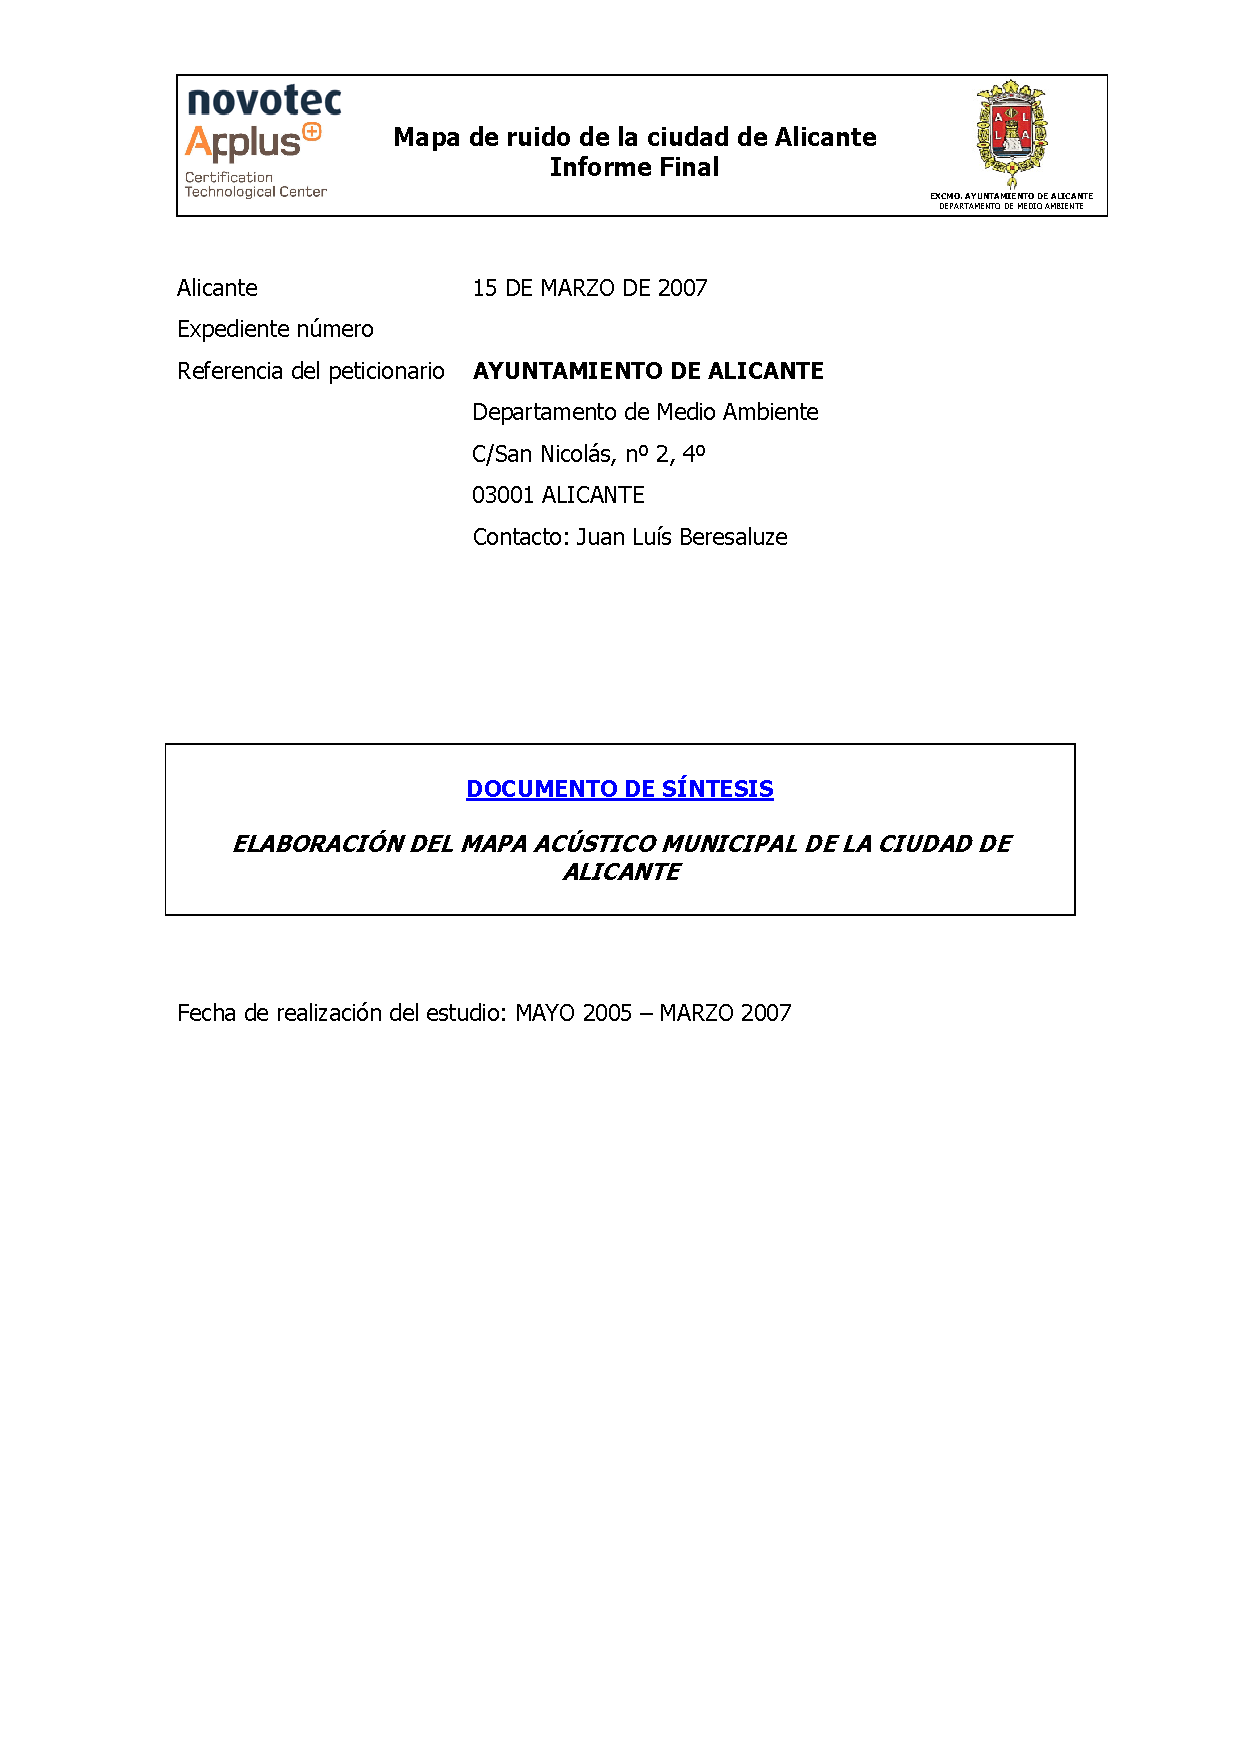
\includepdf[pages={1}]{archivos/ES_a_DF7_Agg_Alicante.pdf}

% Para incluir una página:
% [pages={0}] % Donde '0' es el número de la pagina del PDF que se quiere incluir

% Para incluir varias páginas consecutivas
% [pages={1-4}] % Con estos valores importa de la página 1 a la 4.

% Para incluir varias páginas salteadas
% [pages={1,4,7,10}] % Incluye las páginas 1,4,7 y 10

% Para incluir todo el documento PDF
% [pages=-]

% Si ademas de pages=... se incluye landscape, se importa en horizontal
% [pages{1},landscape]

\end{document}
